\documentclass[../tesis_main.text]{subfiles}


\chapter{Manipulador}
	En esta sección se hablará de las caracteriscias mecánicas del brazo robótico ensamblado en el robot de servicio Justina. Se describirán los elementos que componen el brazo robótico haciendo enfasís en la ubicación de los actuadores y como influye esto en el modelo matematico del mismo. Posteriormente se abordarán los temas respectivos la cinemática de un brazo robótico de 7DOF.\\


%%%%%%%%%%%%%%%%%%%%%%%%%%%%%%%%%%%%%%%%%%%%%%%%%%%%%%%%%%%%%%%%
           %%%%%%  DESCRPCIÓN SERVOMOTORES   %%%%%%%%
%%%%%%%%%%%%%%%%%%%%%%%%%%%%%%%%%%%%%%%%%%%%%%%%%%%%%%%%%%%%%%%%
	\section{Descripción hardware}
		Los servomotores Dynamixel son un sistema de actuador inteligente desarrollados con el propósito de funcionar como uniones de conexión en un robot o estructura mecánica. Los servomotores Dynamixel están diseñados para ser modulares y soportar la conexión en cadena en cualquier robot o diseño mecánico. Este tipo de servomotores es popular por los beneficios que ofrece: movimientos robóticos potentes y flexibles.\\

		El conjunto de servomotores Dynamixel son un grupo de actuadores de alto rendimiento con reductor, controlador y un protocolo de comunicación completamente integrados. El estado del actuador se puede leer y monitorear a través de un flujo de paquetes de datos. \cite{dynamixelEpage}\\

		Los servomotores de la marca Dynamixel, cuentan con diferentes gamas de productos de acuerdo a las necesidades de cada proyecto. El brazo robótico referente a este documento está constituido unicamente por motores de la gama MX, de la cual se describen las caracteristicas más sobresalientes a continuación.\\  

			\subsection{Motores dynamixel Serie MX}
		Los actuadores dynamixel de la serie MX pertencen a la última generación de actuadores de la companñia Robotis Dynamixel. Están equipados con un procesador Cortex M3 de 32 bits a 72 mhz, un encoder magnético sin contacto con una resolución 4 veces mayor que la serie AX / RX, además ofrecen una velocidad de comunicación de hasta 3 mbps con el nuevo bus TTL 2.0. Cada servomotor cuenta con la capacidad  de monitorear su velocidad, temperatura, posición del eje, voltaje y carga.\\

		Por otro lado los motores Dynamixel de la seire MX cuentan con la implemntación de un algoritmo de control PID para mantener la posición del eje. Las ganancias del algoritmo de control PID se pueden ajustar individualmente para cada servo, lo que le permite controlar la velocidad y la fuerza de la respuesta del motor. Todos los servos de la serie MX usan un voltaje nominal de 12v. La característica más importante de esta seie de servomotores es que la gestión de la información proveniente del sensor y la ejecución del algoritmo de control de posición son manejados por el microcontrolador integrado del servo. Este enfoque distribuido deja a su controlador principal libre para realizar otras funciones.\\


		En lo que respecta a la parte mecánica, todos los servos DYNAMIXEL son compatibles con una amplia variedad de bridas, acoplamientos y sujetadores lo cual facilita la construcción de cualquier configuración deseada. Este conjunto de elementos mecánicos permite una conexión directa cualquier modelo de servomotores DYNAMIXEL, lo que le permite una gran variedad de configuraciones para cualquier necesidad. Dada la gran variedad de configuraciones, este tipo de elementos de unión y fijación resultó de gran ayuda mecánica al momento de contruir el brazo robótico donde se implentaron los algoritmos descritos en el presente trabajo.\\

		\begin{figure}[h!]
			\begin{center}
			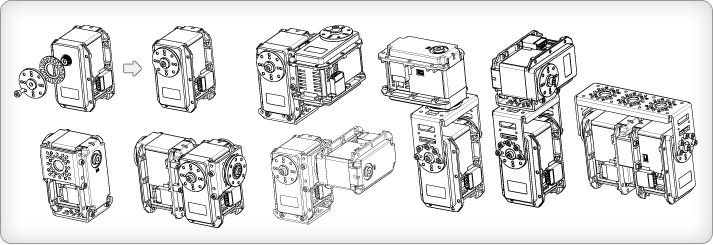
\includegraphics[width=14.5cm, height=6.5cm]{manipulator/dynamixel_conexions.jpg}	
			\caption{Variedad de ensambles para servomotores.}
			\end{center}
		\end{figure}

		Resuminedo las características de los sermovomotores de la serie MX, podemos enlistar las siguientes:\\ 

		\begin{itemize}
			\item{Movimiento sin contacto y detección de posición.}
			\item{Interfaz de comunicación TTL estándar.}
			\item{Comunicación de alta velocidad de hasta 4.5 Mbps.}
			\item{Control PID para autocorrección en posicionamiento.}
			\item{Control de par basado en corriente (4096 steps, 2.69mA/step)}
			\item{Ahorro de energía (corriente reducida de 100 mA a 40 mA)}
		\end{itemize}

		Si desea controlar este servo DYNAMIXEL desde un equipo de computo es necesario contar con un dispositivo que facilite la comunicación entre este y el microprocesador de cada uno de los servomotores, el dispositivo que cumple con esta funcionalidad es el USB2Dynamixel.\\

		El controlador USB2Dynamixel se conecta al puerto USB en una computadora y tiene un puerto de 3 y 4 pines para conectar Dynamixels. El USB2Dynamixel se puede usar con controladores como CM-5 y CM-2 que usan comunicación en serie, además soporta la comunicación en cadena propia de los servomotores Dynamixel. Es impornate mencionar que este dispositivo posee un interruptor para seleccionar entre diferentes protocolos de comunicación: RS-232, RS-485, TTL. Por tanto consta de:\\

		\begin{itemize}
			\item{Conector 3P: puerto de comunicación para nivel TTL (para control de serie AX y MX)}
			\item{Conector 4P: puerto de comunicación RS-485 (para control de serie DX, RX, EX y MX)}
		\end{itemize}


		\begin{figure}[h!]
			\begin{center}
			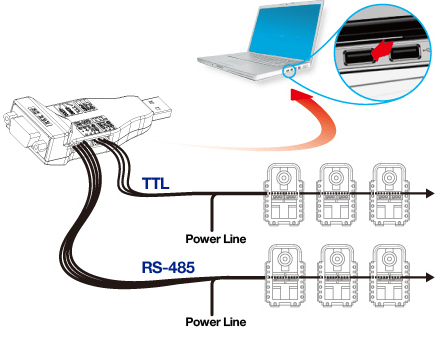
\includegraphics[width=10.5cm, height=8.5cm]{manipulator/usb2dynamixel.jpg}	
			\caption{Dispositivo de comunicación USB a protocolo serial.}
			\end{center}
		\end{figure}

		Los motores que componen esta gama comparten caracteristicas, las cuales se menacionan a continuación:\\

\begin{table}[h!]
\centering 
\begin{tabular}{ |p{6.5cm}||p{2.1cm}|p{2.1cm}|p{2.1cm}|  }
 \hline
 \multicolumn{4}{|c|}{\textbf{MOTORES GAMA MX} } \\
 \hline
 Voltaje de operación  &  14.8v   &	   12v   &   11.1v\\
 \hline
 Protocolo             &  \multicolumn{3}{|c|}{TTL Serial Asincrono} \\
 \hline
 Velocidad del puerto  &  \multicolumn{3}{|c|}{8000bps - 3Mbps} \\
 \hline
 Retroalimentación de posición & \multicolumn{3}{|c|}{ SI} \\
 \hline
 Retroalimentación de temperatura & \multicolumn{3}{|c|}{ SI}\\
 \hline
 Control PID           & \multicolumn{3}{|c|}{ SI } \\
 \hline
 Material              & \multicolumn{3}{|c|}{ Carcasa platica y reducción metálica} \\
 \hline
 Motor                 & \multicolumn{3}{|c|}{ Maxon RE-MAX} \\
 \hline
\end{tabular}
\caption{Características servomotores MX.}
\label{t_manip:1}
\end{table}

		Los modelos de motores que componen esta gama difieren en caracteríticas tales como las dimensiones, el par máximno a rotor bloqueado, la corriente máxima, o la velocidad máxima. A continuación se en listan las características más sobresalientes para cada modelo de motor.\\ 


\newpage
%%%%%%%%%%%%%%%%%%%%%%%%%%%%%%%%%%%%%%%%%%%%%%%%%%%%%%%%%%%%%%%%%%
		\subsection{Características MX-106}
%%%%%%%%%%%%%%%%%%%%%%%%%%%%%%%%%%%%%%%%%%%%%%%%%%%%%%%%%%%%%%%%%%

\begin{table}[h]
\centering
\begin{tabular}{ |p{6.5cm}||p{2.1cm}|p{2.1cm}|p{2.1cm}|  }
 \hline
 \multicolumn{4}{|c|}{\textbf{MX-106} } \\
 \hline
 Voltaje de operación  &  14.8v   &	   12v   &   11.1v\\
 \hline
 Par de bloqueo        &  102kg.cm  &  85.6kg.cm  &  81.5kg.cm\\
 Velocidad sin carga   &  55rpm     &  45rpm      &  41rpm\\
 \hline
 Peso                  &  \multicolumn{3}{|c|}{153g} \\
 \hline
 Tamaño                &  \multicolumn{3}{|c|}{40.2 x 65.1 x 46 mm} \\
 \hline
 Resolución            &  \multicolumn{3}{|c|}{ 0.088 grado/valor de registro} \\
 \hline
 Relación de reducción &  \multicolumn{3}{|c|}{1/200} \\
 \hline
 Corriente máxima      &  \multicolumn{3}{|c|}{5.2A @ 12V} \\
 \hline
\end{tabular}
\caption{Características dynamixel modelo MX-106.}
\label{t_manip:2}
\end{table}


\begin{figure}[h!]
	\begin{center}
	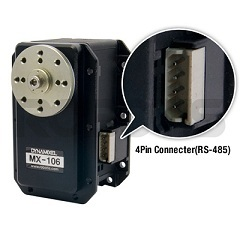
\includegraphics[width=8.5cm, height=8.5cm]{manipulator/MX_106R_2.jpg}	
	\caption{Servomotor dynamixel modelo MX-106.}
	\end{center}
\end{figure}


\newpage
%%%%%%%%%%%%%%%%%%%%%%%%%%%%%%%%%%%%%%%%%%%%%%%%%%%%%%%%%%%%%%%%%%
		\subsection{Características MX-64}
%%%%%%%%%%%%%%%%%%%%%%%%%%%%%%%%%%%%%%%%%%%%%%%%%%%%%%%%%%%%%%%%%%
\begin{table}[h]
\centering
\begin{tabular}{ |p{6.5cm}||p{2.1cm}|p{2.1cm}|p{2.1cm}|  }
 \hline
 \multicolumn{4}{|c|}{\textbf{MX-64} } \\
 \hline
 Voltaje de operación  &  14.8v   &	   12v   &   11.1v\\
 \hline
 Par de bloqueo        &  74kg.cm   &  61kg.cm   &  56kg.cm\\
 Velocidad sin carga   &  78rpm     &  63rpm     &  58rpm\\
 \hline
 Peso                  &  \multicolumn{3}{|c|}{126g} \\
 \hline
 Tamaño                &  \multicolumn{3}{|c|}{40.2 x 61.1 x 41 mm} \\
 \hline
 Resolución            &  \multicolumn{3}{|c|}{ 0.088 grado/valor de registro} \\
 \hline
 Relación de reducción &  \multicolumn{3}{|c|}{1/200} \\
 \hline
 Corriente máxima      &  \multicolumn{3}{|c|}{4.1A @ 12V} \\
 \hline
\end{tabular}
\caption{Caracteríisticas Dynamixel modelo MX-64}
\label{t_manip:3}
\end{table}

\begin{figure}[h!]
	\begin{center}
	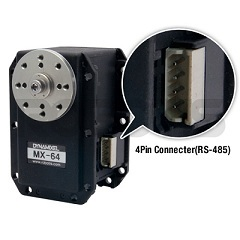
\includegraphics[width=8.5cm, height=8.5cm]{manipulator/MX_64R_2.jpg}	
	\caption{Servomotor dynamixel modelo MX-64.}
	\end{center}
\end{figure}



\newpage
%%%%%%%%%%%%%%%%%%%%%%%%%%%%%%%%%%%%%%%%%%%%%%%%%%%%%%%%%%%%%%%%%%
		\subsection{Características MX-28}
%%%%%%%%%%%%%%%%%%%%%%%%%%%%%%%%%%%%%%%%%%%%%%%%%%%%%%%%%%%%%%%%%%
\begin{table}[h]
\centering
\begin{tabular}{ |p{6.5cm}||p{2.1cm}|p{2.1cm}|p{2.1cm}|  }
 \hline
 \multicolumn{4}{|c|}{\textbf{MX-28} } \\
 \hline
 Voltaje de operación  &  14.8v   &	   12v   &   11.1v\\
 \hline
 Par de bloqueo        &  31.6kg.cm  &  25.5kg.cm   &  23.4kg.cm\\
 Velocidad sin carga   &  67rpm      &  55rpm       &  50rpm\\
 \hline
 Peso                  &  \multicolumn{3}{|c|}{72g} \\
 \hline
 Tamaño                &  \multicolumn{3}{|c|}{35.6 x 50.6 x 35.5 mm} \\
 \hline
 Resolución            &  \multicolumn{3}{|c|}{ 0.088 grado/valor de registro} \\
 \hline
 Relación de reducción &  \multicolumn{3}{|c|}{1/193} \\
 \hline
 Corriente máxima      &  \multicolumn{3}{|c|}{1.4A @ 12V} \\
 \hline
\end{tabular}
\caption{Caracteríisticas Dynamixel modelo MX-64}
\label{t_manip:4}
\end{table}

\begin{figure}[h!]
	\begin{center}
	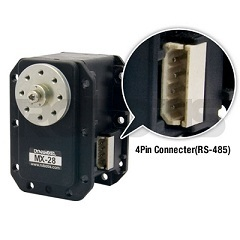
\includegraphics[width=8.5cm, height=8.5cm]{manipulator/MX_28R_2.jpg}	
	\caption{Servomotor dynamixel modelo MX-64.}
	\end{center}
\end{figure}

	Por otro lado es importante conocer la estructura de transmisión de la información de un servomotor con el dispositivo controlador. Para ello los servomotores dynamixel cuentan con un protocolo de comunicación serial asincrono, el cúal transtite una serie de datos en una trama, como se ilustra en la figura[].\\

	\begin{figure}[h!]
		\begin{center}
		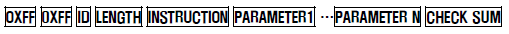
\includegraphics[width=15.5cm, height=1.5cm]{manipulator/trama.png}
		\end{center}
	\end{figure}

	El significado de cada byte que compone al paquete datos es el siguiente:\\

	\begin{itemize}
		\item{ \textbf{0xFF 0xFF} :  Es la instrucción que marca el inicio del paquete.}
		\item{ \textbf{ID} :  Es el ID de cada servomotor partícular en la cadena.}
		\item{ \textbf{LENGTH} :  Es el tamaño del paquete. El tamaño es calculado como el numero de parametros más dos (N+2).}
		\item{ \textbf{INSTRUCTION} :  Indica el tipo de instrucción que ejecutará el servomotor dynamixel.}
		\begin{itemize}
			\item{PING}
			\item{READ\_DATA}
			\item{WRITE\_DATA}
			\item{REG\_WRITE}
			\item{ACTION}
			\item{RESET}
			\item{SYN\_WRITE}
		\end{itemize}
		\item{ \textbf{PARANETER 0...N} :  Este parámetro se usa cuando la instrucción requiere datos auxiliares.}
		\item{ \textbf{CHECK SUM} :  Se usa para verificar si el paquete de datos se dañó durante la comunicación.}
	\end{itemize}
	
	A continuación se anexa una tabla con las caracteriticas más reelevantes de los registros que posee cada uno de los revomotores dynamixel.\\

\begin{table}[H]
\centering
\begin{tabular}{ |p{1.2cm}||p{1.8cm}|p{3.0cm}|p{3.8cm}|p{1.8cm}|  }
 \hline
 \textbf{AREA} &\textbf{Dirección} &\textbf{Nombre} &\textbf{Descripción} &\textbf{Acceso}\\
 \hline
   &  3  &	 ID  &   Identificador del motor & $L/E$\\
 \hline
   &  4  &  Baud Rate  & Velocidad transmisión datos dynamixel & $L/E$\\
 \hline
   &  10 &  Drive mode &  Configuraciones en modo dual  & $L/E$ \\
 \hline
   &  14 & Max Torque(L) & Byte bajo del registro Máx torque & $L/E$\\
 \hline
   &  15 & Max Torque(H) & Byte alto del registro Máx torque & $L/E$\\
 \hline
   &  24 & Torque Enable & On \ Off Torque & $L/E$\\
 \hline
   &  26 & D gain & Ganancia de control derivativa & $L/E$\\
 \hline
   &  27 & I gain & Ganancia de control integral   & $L/E$\\
 \hline
   &  28 & P gain & Ganancia de control proporcional& $L/E$\\
 \hline
   &  30 & Goal position(L) & Byte bajo del registro para una posición deseada & $L/E$\\
 \hline
   &  31 & Goal position(H) & Byte alto del registro para una posición deseada   & $L/E$\\
 \hline
   &  32 & Moving Speed(L) & Byte bajo del registro para una velocidad deseada& $L/E$\\
 \hline
   &  33 & Moving Speed(H) & Byte alto del registro para una velocidad deseada& $L/E$\\
 \hline
   &  34 & Torque Limit(L) & Byte bajo del registro para un par deseado& $L/E$\\
 \hline
   &  35 & Torque Limit(H) & Byte alto del registro para un par deseado& $L/E$\\
 \hline
   &  36 & Present position(L) & Byte bajo del registro de la posición presente& L\\
 \hline
   &  37 & Present position(H) & Byte alto del registro de la posición presente& L\\
 \hline
   &  40 & Present load(L) & Byte bajo del registro de la carga presente& L\\
 \hline
   &  41 & Present load(H) & Byte alto del registro de la carga presente& L\\
 \hline
\end{tabular}
\caption{Tabla de registros para servomotores Dynamixel de la gama MX.}
\label{t_manip:5}
\end{table}

		\subsection{Caracteristicas de conexión}
	Se ha mencionado con anterioridad que el brazo robótico con el cual se realizaron las pruebas correspondientes para este trabajo consta de 10 servomotores dynamixel de la gama MX y de diferentes modelos. Para facilitar la comunicación entre los diferentes modelos de servomotores se utilizó un método de conexión \textit{daysi chain} en cual permite una conexión en cadena entre servomotores, asignandole un ID a cada servomotor y realizando la comunicación a través de un solo puerto.\\

	\begin{figure}[h!]
		\begin{center}
		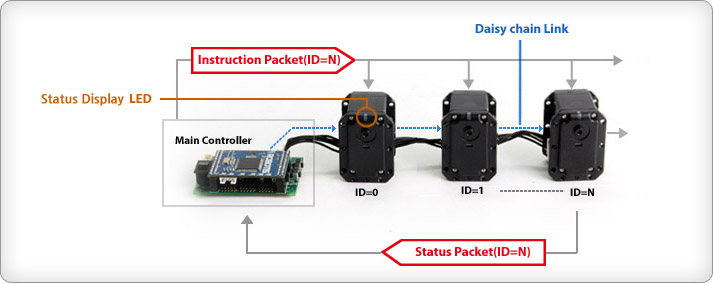
\includegraphics[width=8.5cm, height=4.5cm]{manipulator/dynamixel_daysi_chain.jpg}
		\caption{Servomotores dynamixel en conexión daisy chain.}
		\end{center}
	\end{figure}

	El sistema \textit{daisy chain} es un esquema de conexiones que forman una sucesión de enlaces, tal que el dispositivo A se encunetra conectado al dispositivo B y este, a su vez, se encuentra concectado a un dispositivo C y así sucesivamente. Es importante señalar que en este tipo de conexión los dispositivos no forman redes, en tal caso el dispositivo C no podría estar conectado al dispositivo A. Otro aspecto importante de resaltar es que en este tipo de conexiones al no poder formar redes la comunicación se realiza dispositivo a dispositivo, por tanto los dispositivos ultimos en la cadena pueden presentar retraso o fallas electricas con respecto de los dispositivos primeros en orden de la cadena.\\  


%%%%%%%%%%%%%%%%%%%%%%%%%%%%%%%%%%%%%%%%%%%%%%%%%%%%%%%%%%
%%%%%%%%%%%%%%% DESCRIPCION DEL HARDWARE %%%%%%%%%%%%%%%%%
%%%%%%%%%%%%%%%%%%%%%%%%%%%%%%%%%%%%%%%%%%%%%%%%%%%%%%%%%%

	\section{Descripción de los elementos del sistema de manipulación}
		El sistema de Hardware del brazo robótico está compuesto por un total de 10 servomotores Dynamixel fabricados por la compañía Robotis \cite{dynamixelEpage}. Eta compañia cuenta con diversas gamas de modelos de servomotores según las necesidades de la apliación. A continuación se describirá el sistema en orden descendente.\\

		En la parte superior del brazo robótico se encuentran dos servomotores Dynamixel MX-106 conectados como maestro-esclavo, configurados en este modo trabajan de manera conjunta aumentando el par unitario de cada uno de los servomotores. Dadas las caracteristicas antes descritas en la tabla \ref{t_manip:2}  podemos observar que la configuración de servomotores entrega un par de torsión máximo a rotor bloqueado de $16.8N.m$ @ 12V. El sentido de giro positivo del arreglo de servomotores es el mostrado en la figura[4.8]. \\

		\begin{wrapfigure}{l}{0.60\textwidth}
			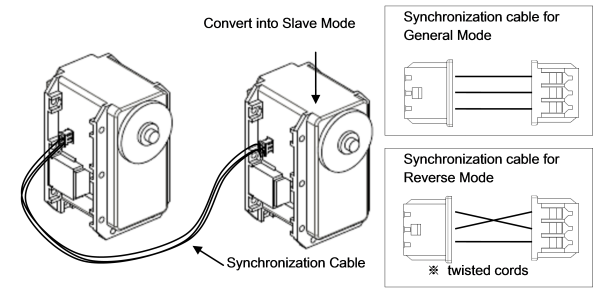
\includegraphics[width=8.0cm, height=4.5cm]{manipulator/mx106_MS.png}
			\caption{Configuración maestro-esclavo en servomotores dynamixel.}
		\end{wrapfigure}

		La configuración maestro-esclavo es un método de control simultaneo para dos servomotores Dynamixel, esta configuración es sumamente útil cuando se trata de construir una junta cuyo eje de acción es coincidente. Los motores respectivos maestro y esclavo deben estar conectados mediante un cable de sincronización. como se muestra en la figura[4.7]. El servomotor esclavo es directamente controlado por la señal PWM del maestro transmitida a travez del cable de sincronización. Es importante mencionar que la información de la posición, velocidad y corriente deseada es ignorada; puesto que esta información depende unicamente del maestro.\\  


		En la configuración maestro-esclavo el esclavo puede configurarse para adoptar un sentido de giro inverso en caso que el acoplamiento mecánico así lo requiera. Dentro de este modo el servomotor esclavo tendrá la misma velocidad que el motor maestro, solo diferenciado por el sentido inverso de giro.\\

		Posteriormente se encuentra un servomotor modelo MX-106, ubicado en una disposición horizontal. Unido a este servomotor se encuentra un eslabón obtenido mediante técnicas de manufactura aditiva. Dado que la construcción del brazo robótico esta pensanda desde el punto de vista antropomórfico  este conjunto de servomotores, el maestro-esclavo y el servomotor MX-106 describen los grados de libertad que emulan el movimiento de un hombro humano.\\

		\begin{wrapfigure}{r}{0.30\textwidth}
			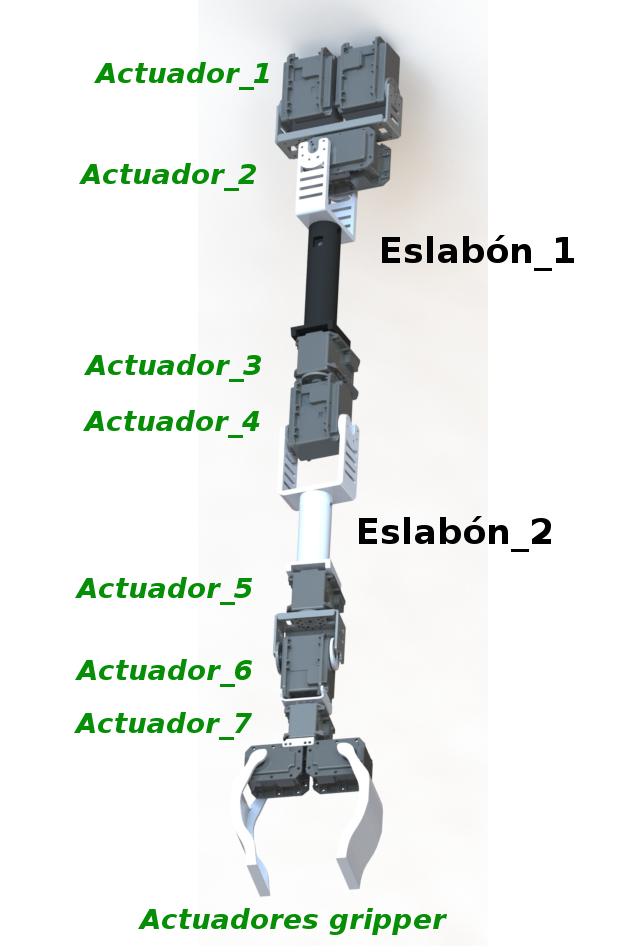
\includegraphics[width=4.5cm, height=12.5cm]{manipulator/brazo_4.jpg}
			\caption{Diseño asistido por computadora del brazo robótico del robot Justina.}
		\end{wrapfigure}

		El eslabón numero 1 obtenido mediante técnicas de manufactura aditiva funge como elemento de unión entre servomotores. Este elemento de unión cuenta con un peso total de **** Al final de este elemnto de unión se encuentra un servomotor MX-64 cuyo eje de acción es perpendicular respcto a la base el brazo. Directamente acoplado a este servomotor se encuentra otro servomotor modelo MX-106. Estos dos servomotores realizan el símil con un codo humano.\\

		Continuando en orden descendente, se encuentra un segundo eslabón utilizado como elemento de unión. En el extremo de este elemento se encuentra un servomotor MX-106, posteriormente un MX-64 y por último un servomoto modelo MX-28. Estos tres elementos construyen un sistema similar al de la muñeca de un brazo humano.\\

		Por último, se encuentra el efector final compuesto de dos actuadores MX-28 ubicados en disposición horizontal. En el eje de acción de cada uno de estos se encuentra una pieza obtenida mediante impresión 3D que funge como sujetador para manipular objetos.\\

		Como podemos observar el brazo robótico consta de un total de 10 servomotores conectados en \textit{daisy chain}.
	

%%%%%%%%%%%%%%%%%%%%%%%%%%%%%%%%%%%%%%%%%%%%%%%%%%%%%%%%%%%%%%%%
              %%%%%%  CINEMATICA DIRECTA   %%%%%%%%
%%%%%%%%%%%%%%%%%%%%%%%%%%%%%%%%%%%%%%%%%%%%%%%%%%%%%%%%%%%%%%%%
\newpage

	\section{Cinemática directa}
El problema de cinemática directa consiste en conocer la posición \textit{(x, y, z)} del efector final dada una determinda configuración de ángulos para el conjunto de actuadores que forman el sistema mecánico. Para ello se describe lo posición del efector final en términos de las transformaciones existentes entre este y la base fija del manipulador.\\


	\subsection{Teoría trasformaciones y medidas del brazo robotico}
	Se partió del sistema mecánico previamente construido del brazo robótico del robot de servicio Justina. Para ello se realizaron mediciones de distancias entre los respectivos ejes de acción de cada uno de los actuadores a fin describir los desplazamientos de los sistemas de refencia en el brazo robótico.\\

	% #####################################################
	% #####################################################
	% ########   Foto brazo real con medidas\\


	Es importante mencionar que para la descripcion de las transformaciones en sistema ROS, podemos contruir la matriz de rotación de tal manera que incluyamos las rotaciones y desplazamientos en los tres ejes coordenados. Esta caracteristica nos proporciona una ventaja sobre los técnicas de descripción de cinematica directa convencionales, tal es el caso del Método Denavith-Hartemberg donde el sistema de transformaciónes debe ser descrito utilizando, unicamente, dos rotaciones y dos translaciones según sus convenciones.\\

	Es importante mencionar esta característica puesto que en algunos casos la concención Denavith-Hartemberg encuentra limitaciones para describir algunas transformaciones arbitrarias. En la representación Denavith-Hartemberg solo hay cuatro parámetros. Pues, mientras que el sistema de referencia i esté rígidamente unido al enlace i, tenemos la libertad para elegir el origen y los ejes de coordenadas del sistema de referencia i+1.\\ 

	Claramente, no es posible representar una transformación homogénea arbitraria usando solo cuatro parámetros. Por lo tanto, comenzamos por determinar qué transformaciones homogéneas se pueden expresar en la forma D\_H.\\

	Supongamos que tenemos dos marcos, indicados por los cuadros 0 y 1, respectivamente. Entonces existe una única matriz de transformación homogénea A que toma las coordenadas del sistema de referencia 1 y las expresa en términos del sistema de referencia 0. Ahora, es necesario aclarar que los sistemas de referencia deben tener dos características adicionales:\\

	\begin{itemize}
		\item{(DH1):  El eje x1 es perpendicular al eje z0}
		\item{(DH2):  El eje x1 intersecta el eje z0} \cite{spong2008robot}\\
	\end{itemize}


    \begin{equation}
	\begin{split}
		T^{n-1}_n = T_{Z_{n-1}}(d_n) * 
			R_z(\theta_n)*T_{x_n} (a_n) * R_{x_n}(\alpha)
    \end{split}
    \end{equation}

    \begin{equation}
	\begin{split}
		T^{n-1}_n = 
		\begin{bmatrix}
\cos \theta_n & -\sin \theta_n \cos \alpha_n & \sin \theta_n \sin \alpha_n &  a_n \cos \theta_n \\
\sin \theta_n & \cos \theta_n \cos \alpha_n & -\cos \theta_n \sin \alpha_n &  a_n \sin \theta_n \\
0     & \sin \alpha_n & \cos \alpha_n &  d_{n} \\
0     &       0        &         0      &    1
		\end{bmatrix}
    \end{split}
    \end{equation}

	Como podemos observar, en la convención de transformaciones Denavith-Hartemberg unicamente requerimos determinar el valor de cuatro variables, dos rotaciones $(\alpha, \theta)$ y dos translaciones $(a, d)$.\\  


	El sistema de descripción de transformaciones desarrollado por ROS, presenta la ventaja que nos prermite describir la trasformación de una manera más detallada. Sin embargo la solución implementada no siempre suele ser la más óptima, encuanto al manejo de la información por ser una mayor cantidad de datos.\\

	Para ello se parte de la matriz de rotación compuesta roll, pitch, yaw.\\

	\begin{equation}
	\begin{split}
		R^{0}_1 = R_{z, \phi } * R_{y, \theta } * R_{x, \psi }
	\end{split}
    \end{equation}

    \begin{equation}
	\begin{split}
		R^{0}_1 = 
		\begin{bmatrix}
		\cos\phi  & -\sin\phi &  0 \\
		\sin\phi  &  \cos\phi &  0 \\
		0         &     0     &   1
		\end{bmatrix}*
		\begin{bmatrix}
		\cos\theta   &   0   &  \sin\theta \\
		   0         &   1   &  0 \\
		-\sin\theta  &   0   &  \cos\theta
		\end{bmatrix}*
		\begin{bmatrix}
		   1      &     0    &   0\\
		   0      &   \cos\psi   &  -\sin\psi \\
		   0      &   \sin\psi   &  \cos\psi
		\end{bmatrix}\\
    \end{split}
    \end{equation}

    \begin{equation}
	\begin{split}
		=
		\begin{bmatrix}
		   \cos\phi \cos\theta & -\sin\phi \cos\psi - \cos\phi \sin\theta \sin\psi & \sin\phi \sin\psi + \cos\phi \sin\theta \cos\psi\\
		   \sin\phi \cos\theta & \cos\phi \cos\psi + \sin\phi \sin\theta \sin\psi  & -\cos\phi \sin\psi + \sin\phi \sin\theta \cos\psi \\
		   -\sin\theta         & \cos\theta \sin\psi   &  \cos\theta \cos\psi
		\end{bmatrix}
    \end{split}
    \end{equation}

	\begin{figure}[h!]
		\begin{center}
		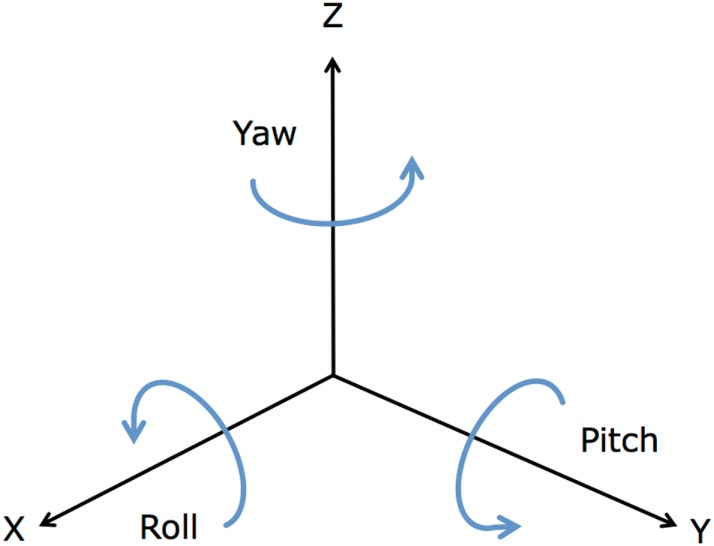
\includegraphics[width=6.5cm, height=4.5cm]{manipulator/roll_pitch_yaw.jpeg}
		\caption{Rotaciones roll, pitch, yaw.}
		\end{center}
	\end{figure} 
    

	\subsection{Implementación (Descrpción con ROS)}

	Se utilizó un visualizador en 3D para observar el modelo del brazo y verificar el correcto movimiento mecánico del brazo. En tal caso se hizo uso de los paquetes proporcionados por \textit{ROS} para la elaboración de modelos de robots. La descrpción del modelo del robot se realizó en una estructura en formato XML. Esta descripción permite describir las transfomaciones existentes entre cada uno de los frames significativos en el robot, así como permite cargar algún modelo \textit{CAD (Computer Assistand Design)} de las piezas que componen al robot.\\

	\begin{figure}[h!]

		\begin{subfigure}[t]{.5\textwidth}
		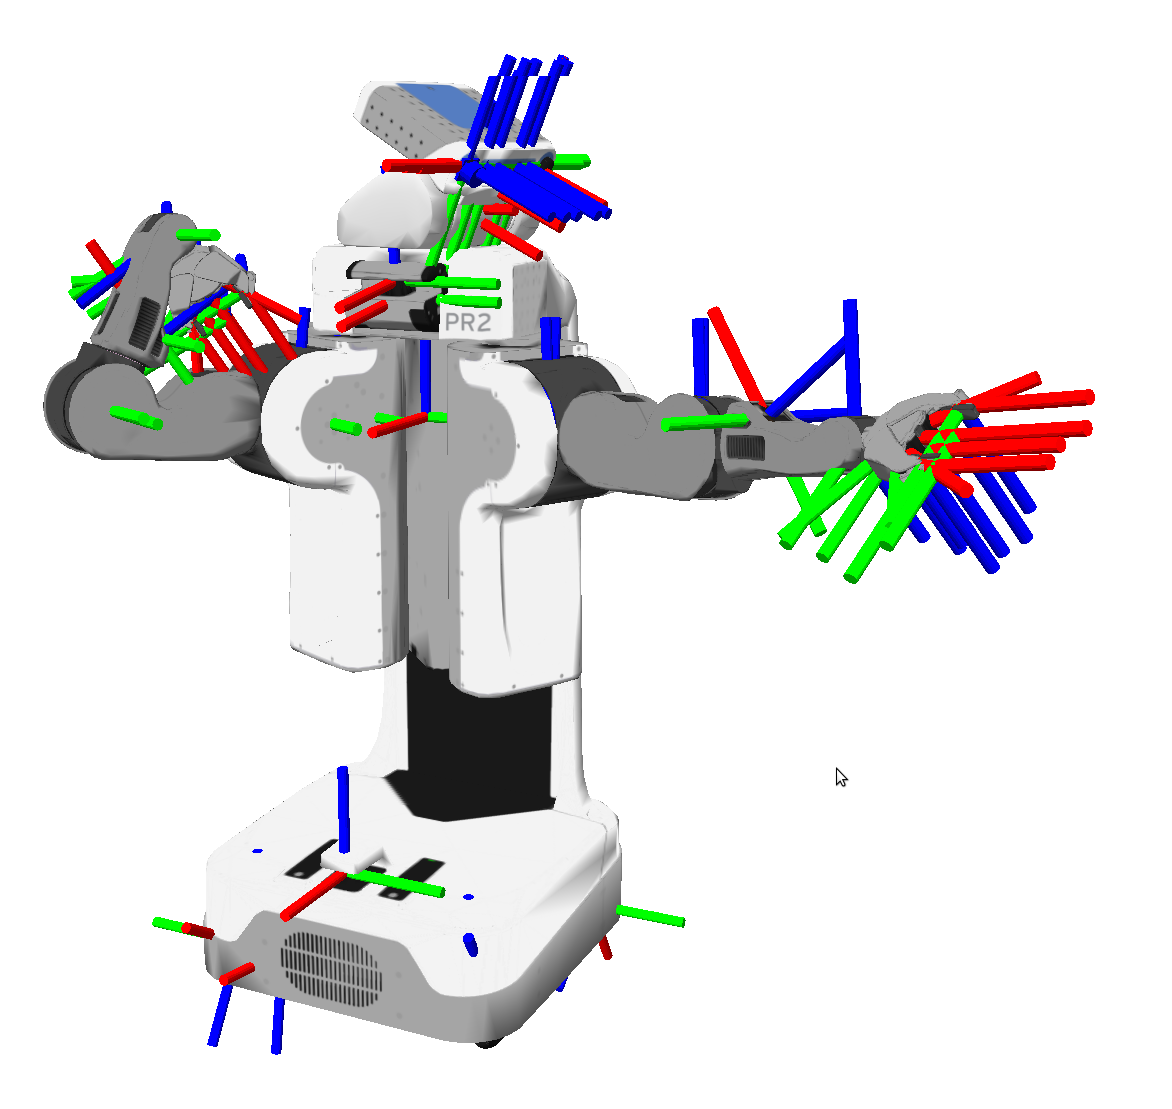
\includegraphics[width=5.5cm, height=5.0cm]{manipulator/tf_example.png}
		\end{subfigure}%
		\begin{subfigure}[t]{.5\textwidth}
		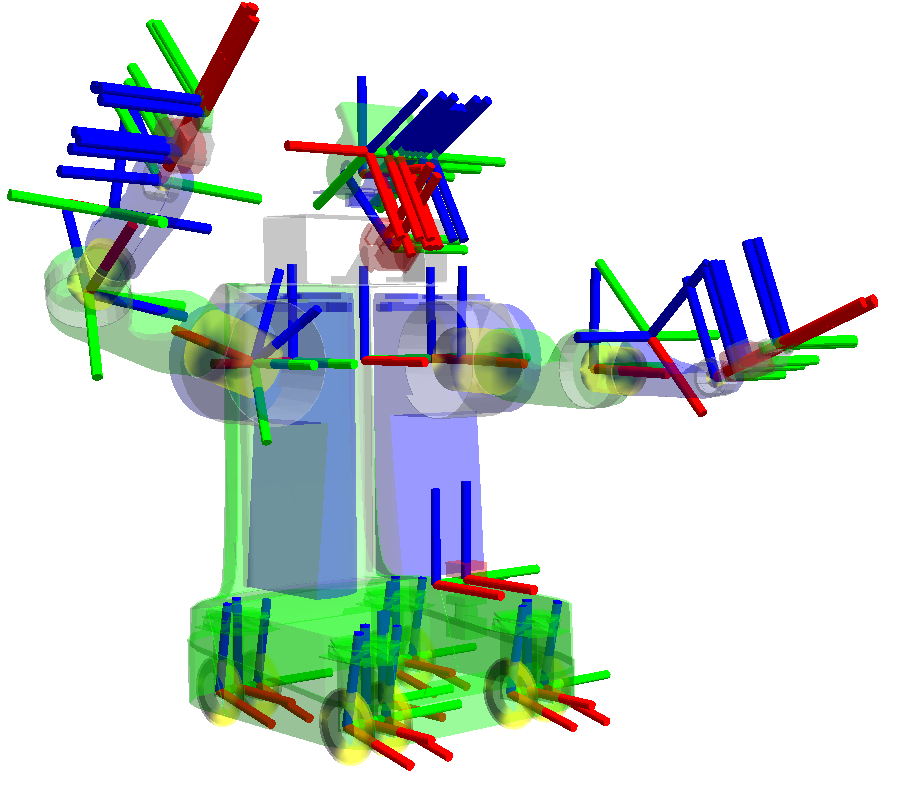
\includegraphics[width=5.5cm, height=5.0cm]{manipulator/tf_example2.png}
		\end{subfigure}

		\caption{Ejemplo de un modelo de robot y sus respectivas transformaciones.}
	\end{figure}



	ROS proporciona una biblioteca de software unicamente dedicada al manejo de información de las transformaciones de un robot, la biblioteca de software lleva el nombre de \textit{tf}. En un nivel práctico, un árbol de transformación define los desplazamientos en términos de translación y rotación entre diferentes marcos de coordenadas. La biblioteca \textit{tf} usa una estructura en árbol para garantizar que solo haya un recorrido único que vincule dos sistemas coordinados entre sí y asume que todas las transformaciones del árbol se dirigen desde los nodos primarios a secundarios.\\ 

	\begin{wrapfigure}{r}{0.45\textwidth}
		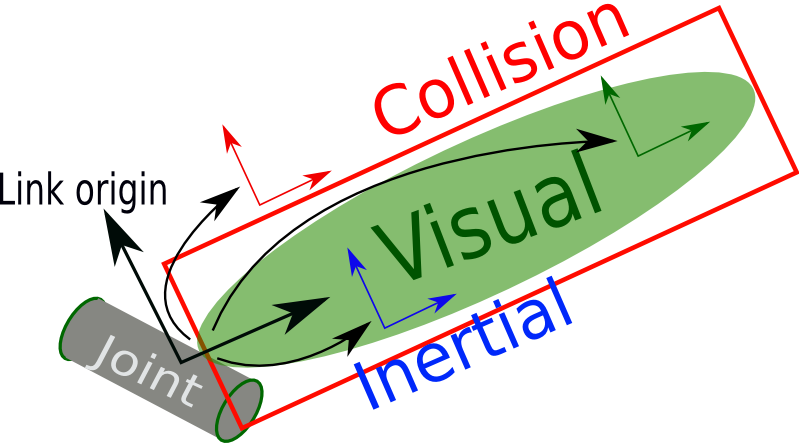
\includegraphics[width=6.5cm, height=3.0cm]{manipulator/link_1.png}
		\caption{Constitución básica de \textit{link} en el sistema ROS.}
	\end{wrapfigure}

	Para describir una transformación se requiere definir primero un conector, que funcione como cada uno de los elementos físicos, posteriormente la transformación se encargará de relacionar cada uno de estos conectores. Conceptualmente, cada nodo en el árbol de transformación corresponde a un sistema de coordenadas el cual representa cada uno de los conectores; por otra parte cada enlace de conexión corresponde a la transformación que debe aplicarse para pasar del nodo actual a su hijo.\\	

	Para crear el árbol de transformaciones del manipulador de 7DOF, comenzamos por crear un sistema de referencia en la base del brazo, el cual servirá como sistema de referencia fijo, lo llamamos \textit{base\_ra\_arm}. Posteriormente se fueron agregando eslabones según la configuración real del brazo. Para llegar a la configuración se partío de la siguiente restricción: el eje Z debe coincidir con el eje de giro del actuador, en posición y en sentido positivo, como se muestra en la figura.\\ 

	\begin{figure}[h!]
		\begin{center}
		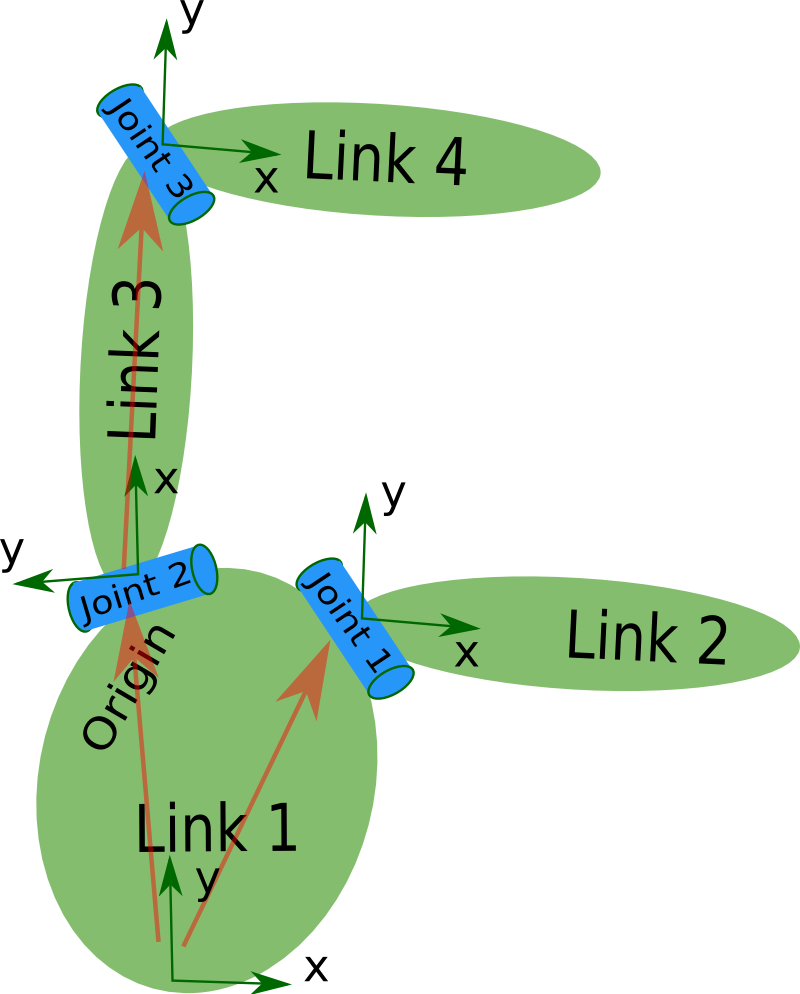
\includegraphics[width=3.5cm, height=4.0cm]{manipulator/link_description.png}
		\caption{Ejemplo de sistema de transformaciones (sistemas de refencia y links).}
		\end{center}
	\end{figure} 

	Para crear esta configuración entre los diferentes sistemas de referencia, primero debemos decidir qué nodo será el padre y cuál será el hijo. Esta distinción es importante porque asume que todas las transformaciones se mueven de padres a hijos. Elegimos el sistema de referencia \textit{base\_ra\_arm} como principal, ya que a medida que se agregan otras piezas: motores, eslabones y conectores, tendrá más sentido que se relacionen con un sistema fijo. Esto significa que la transformada asociada con el efector final y el sistema \textit{base\_ra\_arm} puede ser obtenida mediante el árbol de transformaciones configurado. La conversión de la posición del sistema de refencia ubicado en el efector final al sistema de referencia fijo ubicado en la base del brazo puede ser obtenida mediante una llamada a la biblioteca tf.\\

	\subsection{Comparación cinemática directa Denavith-Hartemberg y cescripción completa de transformaciones}

	Se implementaron dos metodologías de descripciones para el cálculo de la cinemática directa del brazo robótico. La primera de ellas consistió en realizar la descripción completa de las tranfomaciones utilizando la información de rotación y translación de cada uno de los respectivos sistemas de referencia.\\

	En este proceso y con la información previamente obtenida de las dimensiones del brazo robótico se construyó la siguienta tabla donde se muestra la información de los desplazamientos y rotaciones de los respectivos sistemas de referencia.\\

\begin{table}[H]
\centering
\begin{tabular}{ |p{1.0cm}|p{1.5cm}|p{1.5cm}|p{1.5cm}|p{1.5cm}|p{1.5cm}|p{1.5cm}|}
 \hline
  & \multicolumn{3}{|c|}{\textbf{TRANSALACIÓN}} & \multicolumn{3}{|c|}{\textbf{ROTACIÓN}} \\
 \hline
  &  x & y & z & roll & pitch & yaw\\
 \hline
 1 &  0.065 & 0.00 & 0.000 & $\pi /2$  &   0.000   & 0.000    \\
 \hline
 2  & 0.215 & 0.00 & 0.000 &   0.000   & $\pi /2$  & 0.000    \\
 \hline
 3  & 0.000 & 0.00 & 0.060 & $-\pi /2$ & $-\pi /2$ & 0.000    \\
 \hline
 4  & 0.190 & 0.00 & 0.000 & $\pi /2$  &   0.000   & $\pi /2$ \\
 \hline
 5  & 0.000 & 0.00 & 0.036 & $-\pi /2$ & $-\pi /2$ &  0.000   \\
 \hline
 6  & 0.095 & 0.00 & 0.000 & $\pi /2$  &   0.000   & $\pi /2$ \\
 \hline
\end{tabular}
\caption{Tabla de parametros de transformaciones entre sistemas de refencia para el brazo robotico de 7DOF.}
\label{t_manip:6}
\end{table}

	Con la información obtenida de las dimensiones del brazo robótico real pudimos realizar un modelo virtual del brazo utilizando un archivo en formato XML donde describimos las trasfomaciones entre los diferentes sistemas de referencia y los elemetos de conexión obtenidos de modelos CAD. El resultado se puede observar en la figura[4.13]\\ 

	El formato de descrpción virtual de un modelo de robot en formato XML se compone de \textit{links} y \textit{joints}. Un link describe las características de un elemento de unión, estas pueden ser mecánicas, de material, de posición, etc. Un \textit{joint} por otra parte describe la realción existente entre los origenes de dos links, dicho de otro modo decribe la transformación existente entre los sistemas de refencias (\textit{origenes}) de dos links.\\

	\newpage
	\begin{center}
	\begin{lstlisting}[language=html, caption=Descripción parcial del sistema de manipulación]
<link name="base_ra_arm">
    <visual>
      <origin xyz="-0.01 0.0 0.0" rpy="1.5707 0.0 1.5707"/>
      <geometry> 
        <mesh filename="package://knowledge/hardware/stl/brazo/mx106_2.stl"/>
      </geometry>
      <material name="black_gray"><color rgba="0.2 0.2 0.2 1"/></material>
    </visual>
  </link>

  <link name="ra_link0">
    <visual>
      <origin xyz="0.0 0.0 0.005" rpy="0.0 -1.5707 0.0"/>
      <geometry> 
        <mesh filename="package://knowledge/hardware/stl/brazo/mx106_s.stl"/>
      </geometry>
      <material name="gray_black"><color rgba="0.3 0.3 0.3 1"/></material>
    </visual>
  </link>

  <link name="ra_link1">
    <visual>
      <origin xyz="0.0 0.0 0.0" rpy="1.5707 -1.5707 0.0"/>
      <geometry> 
        <mesh filename="package://knowledge/hardware/stl/brazo/bone_1.stl"/>
      </geometry>
      <material name="ra_material"><color rgba="0.9 0.85 0.75 1"/></material>
    </visual>

  </link>
  .
  .
  .
   <joint name="ra_1_joint" type="revolute">
    <origin xyz="0.0 0.0 0.0" rpy="0.0 0.0 0.0"/>
    <parent link="base_ra_arm"/>
    <child link="ra_link0"/>
    <limit effort="0.0" lower="0.0" upper="0" velocity="0.0"/>
    <axis xyz="0 0 1"/>
  </joint>

  <joint name="ra_2_joint" type="revolute">
    <origin xyz="0.064 0.0 0.0" rpy="1.5707 0.0 0.0"/>
    <parent link="ra_link0"/>
    <child link="ra_link1"/>
    <limit effort="0.0" lower="0.0" upper="0" velocity="0.0"/>
    <axis xyz="0 0 1"/>
  </joint>
  .
  .
  .
\end{lstlisting}
\end{center}


	\begin{figure}[H]
		\begin{subfigure}[t]{.5\textwidth}
		\centering
		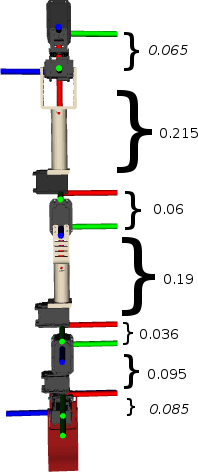
\includegraphics[width=4.2cm, height=8.5cm]{manipulator/brazo_lateralView.png}
		\caption{Vista lateral.}
		\end{subfigure}%
		\begin{subfigure}[t]{.5\textwidth}
		\centering
		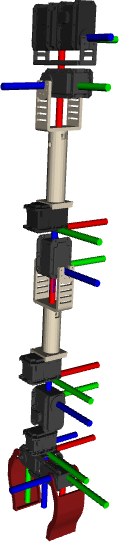
\includegraphics[width=2.2cm, height=8.5cm]{manipulator/brazo_posterior.png}
		\caption{Vista trimetrica.}
		\end{subfigure}
		\caption{Modelo virtual del brazo robótico.}
	\end{figure}	

	Por otro lado se realizó la descripción del sistema de manipulación utilizando la convención Denavith-Hartemberg. Para ello se comenzó por plantear los ejes $z$ que deben ser coincidentes, en posición y en sentido de giro, con los ejes de acción de cada uno de los actuadores. Sin embargo, en este punto se observó una limitante en el método D-H, al intenar describir la trasformación entre el $link_2$ y el $link_3$ se observó que el método no puede describir con suficiente presición la rotación en el eje $"x"$ y al mismo tiempo un desplamiento en el $eje y$. La manera de solucionar esta limittante consiste en realizar una transformación de rotación en el eje x primero, con esto los dos frames compartiran el mismo origen del sistema de referencia, posteriormente se plantea la translación, ahora en el $eje z$.\\
	
	\begin{figure}[h!]
		\begin{center}
		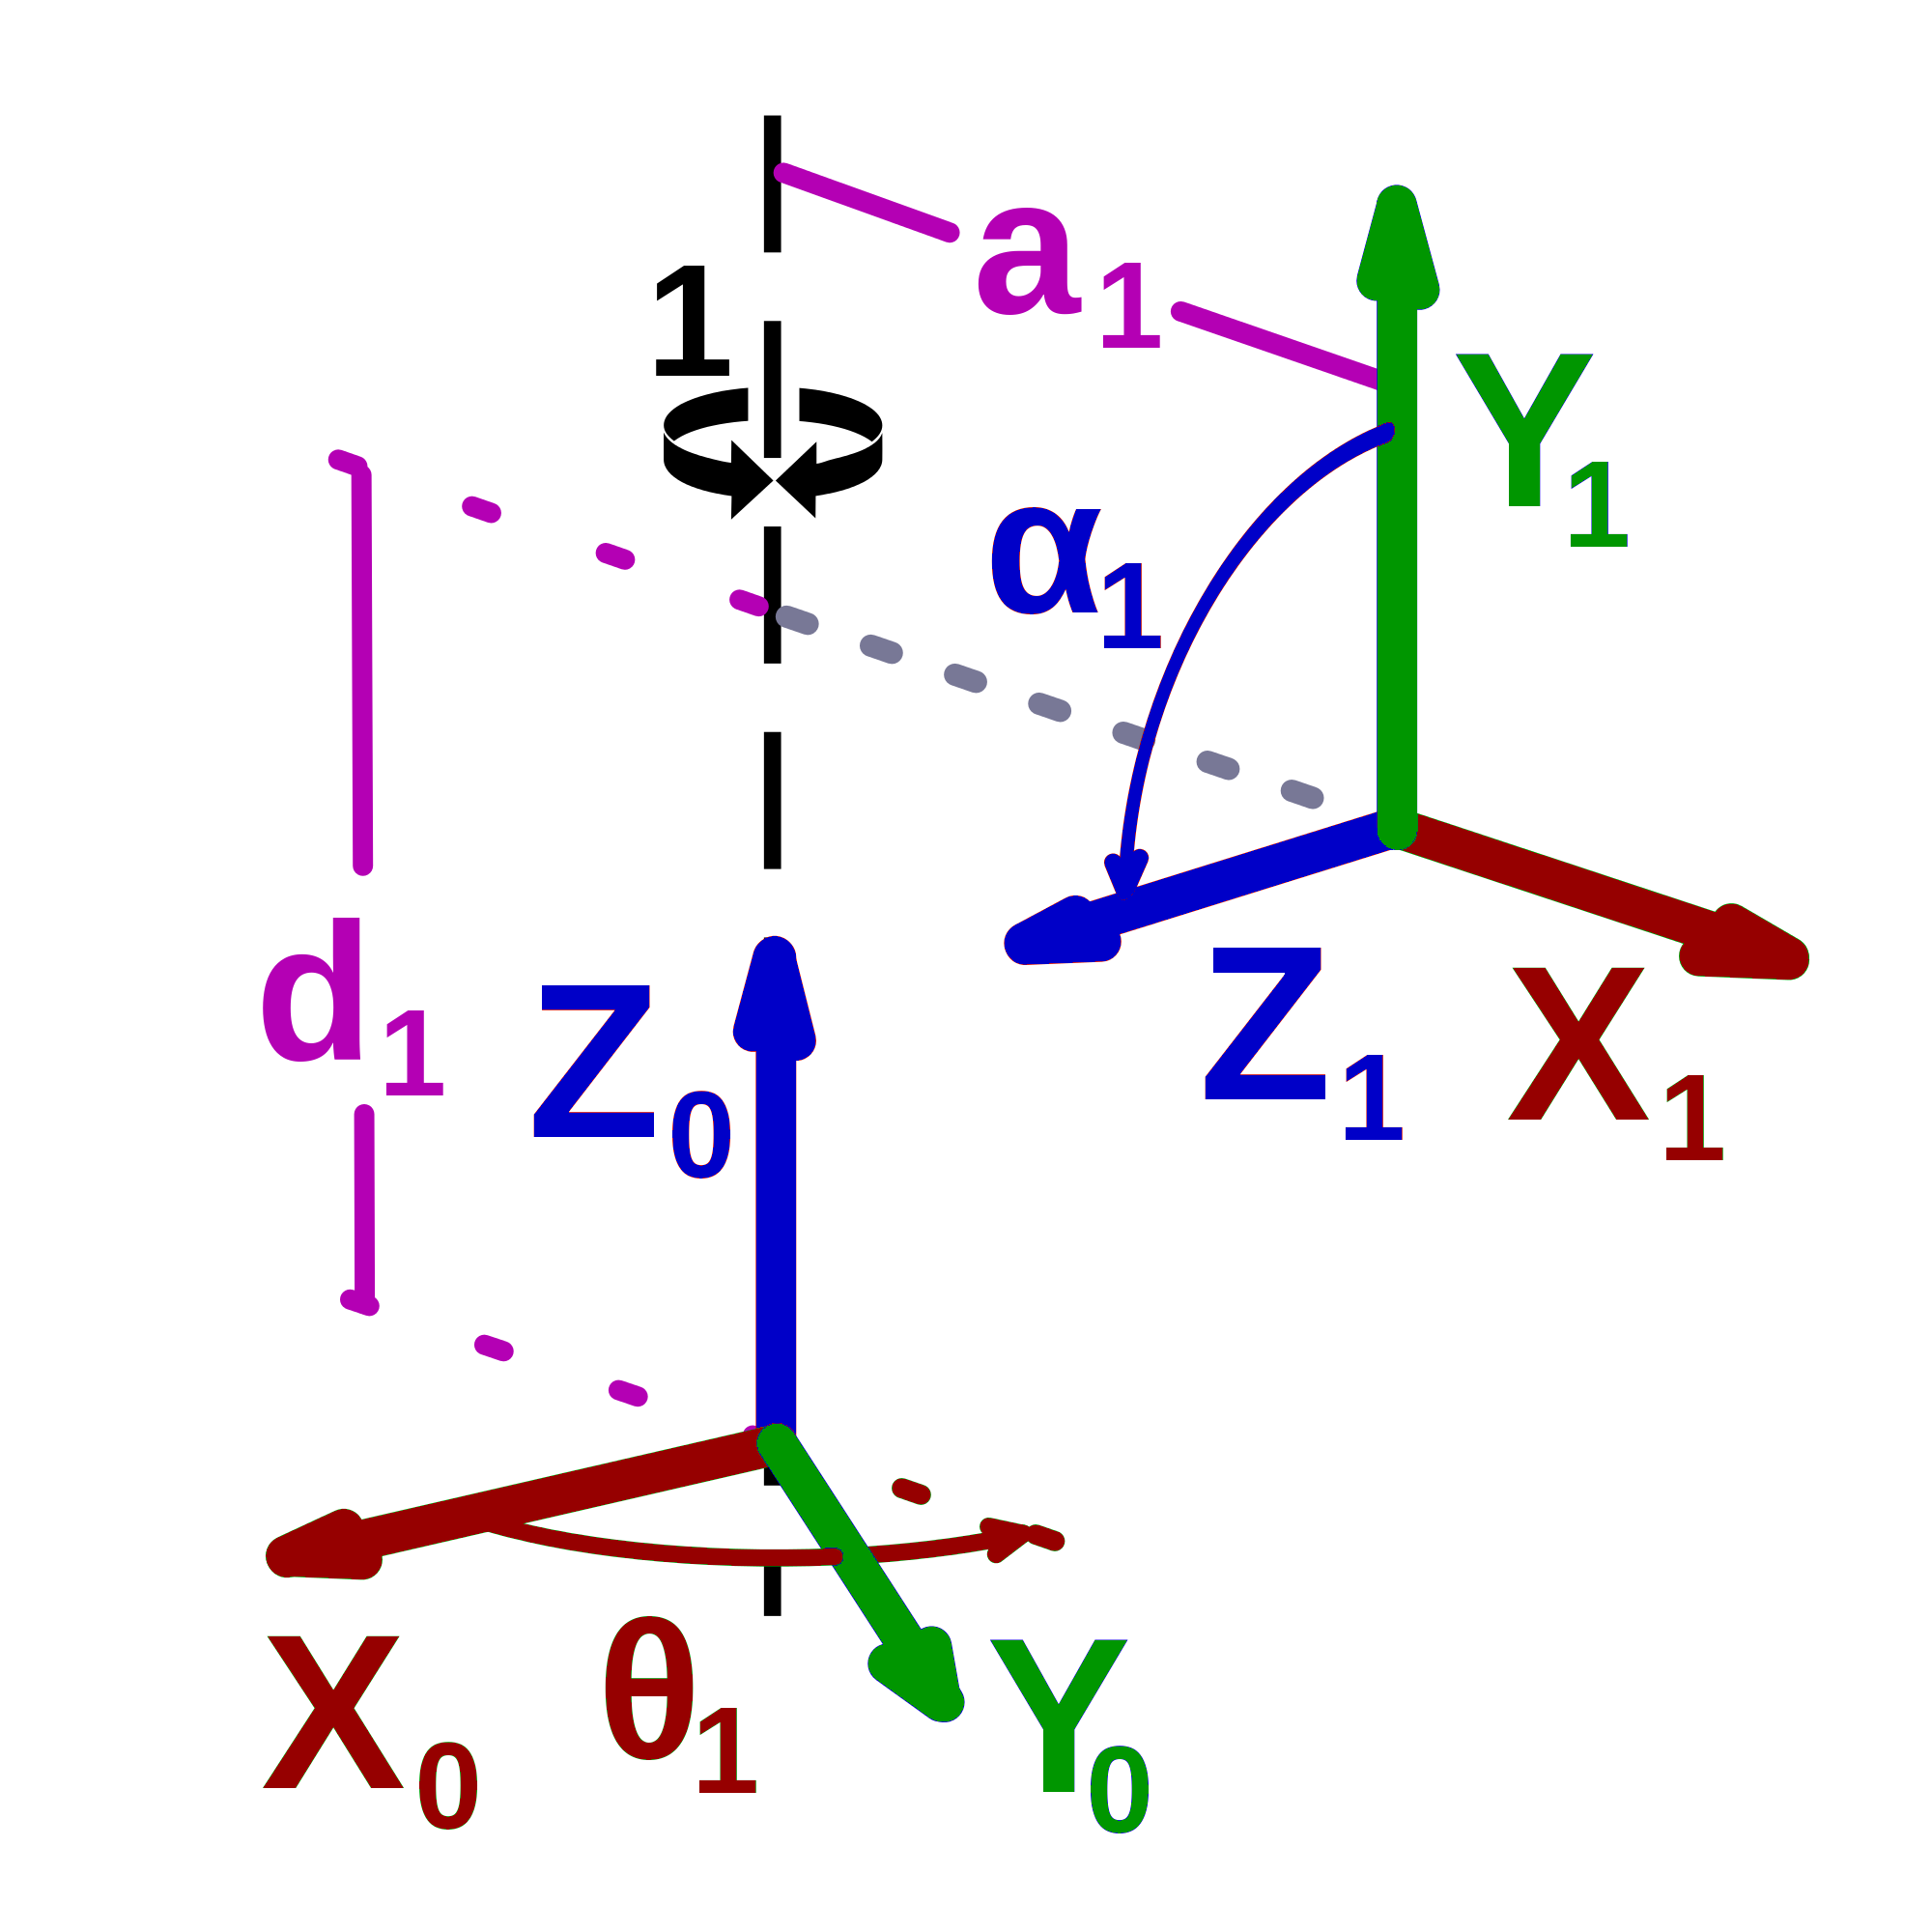
\includegraphics[width=6.5cm, height=6.0cm]{manipulator/DH_transform_ROS.png}
		\caption{Ejemplo de  obtención de parametros DH.}
		\end{center}
	\end{figure} 

	Por tanto, los parámetros que describen las transformaciones del brazo según la convencion D-H, se muestra en la siguiente tabla:\\

\begin{table}[H]
\centering
\begin{tabular}{ |p{1.5cm}|p{1.5cm}|p{1.5cm}|p{1.5cm}|p{1.5cm}|}
 \hline
 \multicolumn{5}{|c|}{\textbf{PARAMETROS DENAVITH-HARTEMBERG}} \\
 \hline
      &    D  &   A   & $\alpha$  &  $\theta$ \\
 \hline
 0-1  & 0.000 & 0.065 & $\pi /2$  &   0.000   \\
 \hline
 1-2  & 0.000 & 0.000 & $\pi /2$  & $\pi /2$  \\
 \hline
 2-3  & 0.275 & 0.000 & $-\pi /2$ & $-\pi /2$ \\
 \hline
 3-4  & 0.000 & 0.000 & $\pi /2$  &   0.000   \\
 \hline
 4-5  & 0.226 & 0.000 & $-\pi /2$ &   0.000   \\
 \hline
 5-6  & 0.000 & 0.000 & $\pi /2$  &   0.000   \\
 \hline
 6-7  & 0.165 & 0.000 &   0.000   &   0.000   \\
 \hline
\end{tabular}
\caption{Tabla de parametros D-H para brazo robotico antropomórfico de 7DOF.}
\label{t_manip:7}
\end{table}

\begin{figure}[H]
	\begin{subfigure}[t]{.5\textwidth}
	\centering
	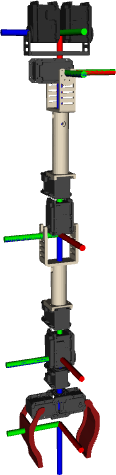
\includegraphics[width=2.5cm, height=8.5cm]{manipulator/DH_1.png}
	\caption{Vista trimétrica.}
	\end{subfigure}%
	\begin{subfigure}[t]{.5\textwidth}
	\centering
	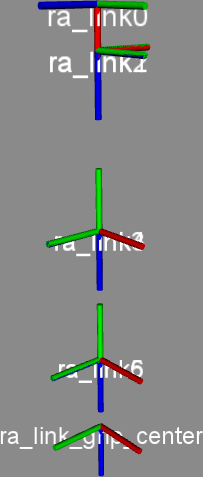
\includegraphics[width=3.50cm, height=8.5cm]{manipulator/DH_3.png}
	\caption{Vista de transformaciones.}
	\end{subfigure}
	\caption{Modelo virtual del brazo robótico utilizando la conveción DH.}
\end{figure}


	Como se puede observar en la Figura 4.14, la descripción de las transformaciones entre el $link 1$ y el $link 2$ comparten el origen. Unicamente difieren en la rotación del respectivo sistema de referencia. Sucede lo mismo para describir la transformación entre las parejas de $links$:  $[3 - 4]$ y $[5 - 6]$.\\

	De la comparación de estas dos representaciones podemos obetener pros y contras de cada una de ellas. Por un lado una representación completa de las trasformaciones nos da la posibilidad de realizar una descripción con mayor presición de cada una de las transformaciones. Esta característica permite alinear cada uno de los sistemas de referencia a el eje de acción de cada uno de los actuadores. En este sentido, es conveniente utilizar esta descripción puesto que simplifica la manera de publicar cada una de las transformaciones entre los sistemas de rerefencia, basta con estar leyendo la posición de cada uno de los actuadores y publicar dicho valor para obtener la representación grafica de la configuración del brazo en el modelo virtual.\\

	Por otro lado, estar escuchando en tiempo real una transformación compuesta de siete trasnformaciones completas requiere un mayor costo computacional comparado con realizar la multiplicación de las mismas siete matrices de transformación solo cuando sea de interés conocer la posición del efector final. En tal caso resulta conveniente tener las dos descripciones: la descripción completa para el despliegue de información de manera visula en el ambiente virtual y la descripción D-H para conocer la posición del efector final cuando sea necesario.\\




%%%%%%%%%%%%%%%%%%%%%%%%%%%%%%%%%%%%%%%%%%%%%%%%%%%%%%%%%%%%%%%%
  %%%%%%%%%%%%%    DETERMINACIÓN DEL WORKSPACE    %%%%%%%%%%%%
%%%%%%%%%%%%%%%%%%%%%%%%%%%%%%%%%%%%%%%%%%%%%%%%%%%%%%%%%%%%%%%%
\newpage
	\section{Determinación del área de trabajo}

	El espacio de trabajo es otro parámetro importante el cual servirá para optimizar las dimensiones del brazo robótico con el cual estamos trabajando. El análisis del espacio de trabajo de robots manipuladores es de gran interés, puesto que la geometría del espacio de trabajo puede considerarse no sólo un aspecto fundamental para el diseño del robot sino que también es esencial para la ubicación del robot en el entorno de trabajo y también para la planificación de trayectorias.\\

	En robótica, el término espacio de trabajo, también denominado espacio de trabajo, puede ser entendido como: \textit{El espacio de trabajo de un robot está definido como el grupo de puntos que pueden ser alcanzados por su efector-final.} \textbf{Cao et al. (2011).}\\

	Dicho de otro modo, el espacio de trabajo de un robot es el espacio en el cual el mecanismo puede trabajar según sus propias restricciones mecánicas. A pesar de que esta definición está muy extendida, diversos autores también se refieren al espacio de trabajo como \textit{volumen de trabajo}.\\

\begin{figure}[H]
	\centering
	\begin{subfigure}[t]{.55\textwidth}
	\centering
	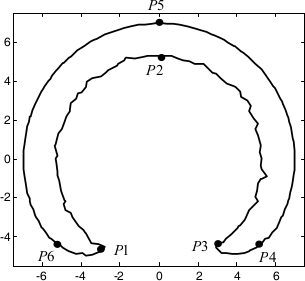
\includegraphics[width=4.5cm, height=4.5cm]{workSpace/ws_Yi_Cao_1.png}
	\caption{Nube de puntos del espacio de trabajo en 2D.}
	\end{subfigure}%
	\begin{subfigure}[t]{.55\textwidth}
	\centering
	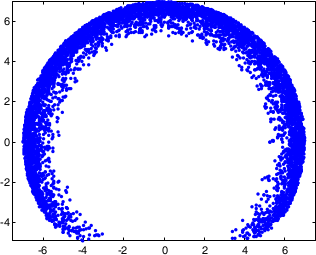
\includegraphics[width=5.00cm, height=4.3cm]{workSpace/ws_Yi_Cao_2.png}
	\caption{Curva de la frontera del espacio de trabajo del brazo robótico.}
	\end{subfigure}
	\caption{Vista en 2D del espacio de trabajo de un robot 3R.}
\end{figure}

	La Figura 4.15 muestra el espacio de trabajo de un robot 3R, donde los puntos  de color azul representan el espacio de trabajo de este robot. Como se ha dicho previamente, los puntos en color azul representan cada una de las posiciones que puede alcanzar el efector-final del robot 3R.\\


\textbf{Principales características de un espacio de trabajo.}

	Cuando se pretende estudiar un espacio de trabajo, lo más importante es su forma y volumen (dimensiones y estructura). Ambos aspectos tienen una importancia significativa debido al impacto que éstos ejercen en el diseño del robot y también en su manipulabilidad. En el presente trabajo se dará una mayor importancia al estudio de las dimensiones del espacio de trabajo desde el punto de vista de la manipulabilidad.\\

	En el caso del presente trabajo fue presciso conocer las características de  forma, dimensiones y estructura del robot a analizar. Puesto que de estas caracteristicas depenederá su espacio de trabajo. 

\begin{itemize}
	\item{La forma es importante para la definición del entorno donde el robot trabajará.}

	\item{Las dimensiones son importantes para la determinación del alcance del efector-final.}

	\item{La estructura del espacio de trabajo es importante para asegurar las características cinemáticas del robot las cuales están relacionadas con la interacción entre el robot y el entorno.}
\end{itemize}

	Además, la forma, dimensiones y estructura del espacio de trabajo dependen de las propiedades del robot en cuestión. Las dimensiones de los eslabones del robot y las limitationes mecánicas de las articulaciones tienen una gran influencia en las dimensiones del espacio de trabajo. La forma depende de la estructura geométrica del robot y también de las propiedades de los grados de libertad. Por otro lado la estructura del espacio de trabajo viene definida por la estructura del robot y las dimensiones de sus eslabones.\\


%%%    ########################################   %%%%%%%%
%%% IMPLEMENTACION: OBTENCIÓN DEL WS DEL BRAZO ROBOTICO
%%%    ########################################   %%%%%%%%

	Para la obtención del espacio de trabajo del brazo robótico en cuentión fue presciso partir de las características antes mencionadas. En este aspecto conocemos las tres características necesarias para la obtención del espacio de trabajo del robot, en cuanto a la forma podemos mencionar que el robot en cuestion es antropomórfico de 7 grados de libertad, cuyas dimensiones las hemos obtenido con anterioridad. En cuanto a la estructura podemos mencionar que conocemos el modelo de la cinemática directa del brazo e incluso que podemos visualizar en tiempo real la configuración del brazo antropomórfico, y por ende conocer la posiçión del efector final. Solo hace falta conocer las restricciones mecánicas del brazo robótico, por tanto se incluye la tabla \ref{t_manip:8} .\\

\begin{table}[H]
\centering
\begin{tabular}{ |p{0.5cm}|p{1.5cm}|p{1.5cm}|}
 \hline
 \multicolumn{3}{|c|}{\textbf{RESTRICCIONES MECÁNICAS }} \\
 \multicolumn{3}{|c|}{\textbf{DEL BRAZO ROBÓTICO}} \\
 \hline
    &  $\theta_1 $ & $[1.47, -1.47]$ \\
 \hline
    &  $\theta_2 $ & $[1.25, -0.21]$ \\
 \hline
    &  $\theta_3 $ & $[1.5707, -1.5707]$ \\
 \hline
    &  $\theta_4 $ & $[2.15, -1.15]$ \\
 \hline
    &  $\theta_5 $ & $[1.5707, -1.5707]$ \\
 \hline
    &  $\theta_6 $ & $[1.5, -1.35]$ \\
 \hline
    &  $\theta_7 $ & $[1.5707, -15707]$ \\
 \hline
\end{tabular}
\caption{Tabla de restricciones mecánicas para brazo robotico antropomórfico de 7DOF.}
\label{t_manip:8}
\end{table}

	Dentro de las metodologías planteadas para la obtención del espacio de trabajo de un robot existen diversas vertientes, una de ellas menciona la posibilidad de obtener dicho espacio generando números aleatorios con una distribución normal acotando los valores aleatorios dentro de las restricciones mecánicas. Posteriormente con los valores aleatorios de ángulos y el modelo de la cinemática directa del brazo robótico obtener la posición del efector final e ir graficando cada uno de estos valores en el tiempo.\\ %%\textbf{****cite}.\\


\begin{figure}[H]
	\centering
	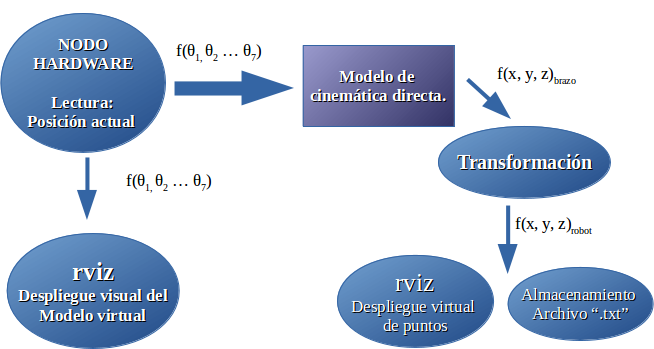
\includegraphics[width=11.00cm, height=7.0cm]{workSpace/esquema_WS2.png}
	\caption{Esquema de construcción del espacio de trabajo para un robot de 7DOF.}
\end{figure}

	Sin embargo, para el desarrollo de este documento se trabajó tanto con el modelo físico del brazo robótico en cuestión, así como con el modelo virtual del mismo. Dadas estas condiciones se planteó el desarrollo de la siguiente manera: con el modelo físico del brazo se obtuvieron en tiempo real las lecturas de posición de cada uno de los actuadores, posteriormenete se actualizaba el modelo virtual del mismo. Con esta información previa, los valores de posición de cada uno de los actuadores y el modelo de la cinemática directa del brazo, se calculaba en tiempo real la posción del efector final. Dicho de otra manera se realizó una construcción en tiempo real del espacio de trabajo del robot.\\

\begin{figure}[H]
	\centering
	\begin{subfigure}[t]{.55\textwidth}
	\centering
	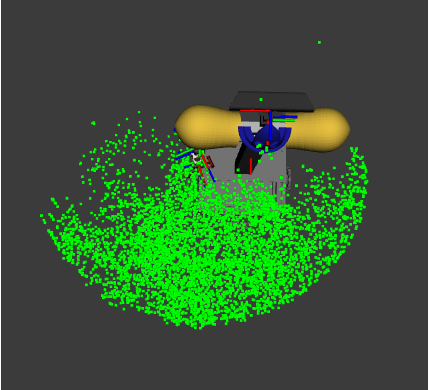
\includegraphics[width=4.50cm, height=4.5cm]{workSpace/ws_9.png}
	\caption{Vista superior.}
	\end{subfigure}%
	\begin{subfigure}[t]{.55\textwidth}
	\centering
	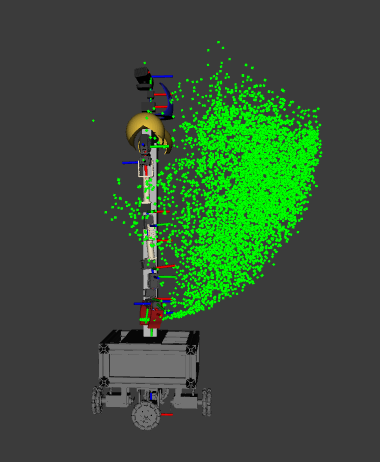
\includegraphics[width=4.20cm, height=4.5cm]{workSpace/ws_8.png}
	\caption{Vista lateral.}
	\end{subfigure}
	\caption{Nube de puntos del espacio de trabajo de un robot antropomórfico de 7DOF.}
\end{figure}

	La ventaja que esta técnica supone, sobre otras, es la capacidad de obtener el espacio de trabajo tomando en cuenta la restricciones reales del robot, así como observar las trayectorías y los puntos críticos del efector final. En este sentido es importante mencionar que para algunos casos el efector final podría alcalzar un punto dentro del área de trabajo; sin embargo dada alguna configuración del brazo esta podría suponer un esfuerzo indeseado en alguno de los actuadores. Con esta técnica se pudo evitar ese tipo de configuraciones, y construir el espacio de trabajo bajo estos supuestos.\\

	Se obtuvo la nube de puntos que en forma se puede aproximar a la sección de una esfera, como se observa en la figura [4.18] . En el desarrollo de este trabajo se planteó la problemática de conocer si el brazo robotico es capáz de alcanzar un punto especifíco en el espacio, en tal caso los desarrollos en este punto deberían abordar la tematica de la siguiente manera: encontrar la ecuación de un volumen que se aproxime a la forma que posee la nube de puntos con el objetivo de saber con certeza si el punto pertenece al volumen de trabajo del manipulador.\\

	El problema de concocer aquellos puntos alcanzables para el brazo robótico, se abordó de la siguinete manera, se propuso una región en el espacio con forma prismatica. La región en el espacio mencionada con anterioridad cumple la condición que sus vertices pertenecen a la nube de puntos del espacio de trabajo del robot, con esto se asegura que todos los puntos dentro de la región propuesta son alcanzables para el robot.\\ 

	Sin perder de vista el objetivo final de este trabajo que es la correcta manipulación de objetos con cierta rotación en "z", este objetivo anañade una limitante más: \"La región en el espacio propuesta debe contener puntos donde el efector final pueda llegar con una orientación en $z$  de por lo menos $\pi/2$ respecto sistema de referencia del robot\". Para ello restamos a el valor máximo en el eje "x" del espacio de trabajo la cantidad $0.165[m]$ según los parametros DH. De esta manera se consiguió obtener un espacio de trabajo acotado cuyas caracteristicas se observan en la figura [4.19] y en la tabla [4.9].\\

\begin{figure}[H]
	\centering
	\begin{subfigure}[t]{.55\textwidth}
	\centering
	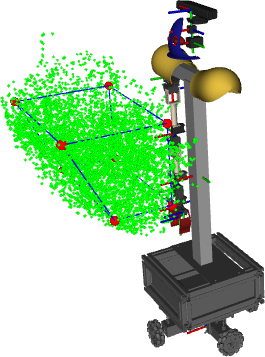
\includegraphics[width=4.50cm, height=5.5cm]{workSpace/ws_bb11.png}
	\caption{Vista superior.}
	\end{subfigure}%
	\begin{subfigure}[t]{.55\textwidth}
	\centering
	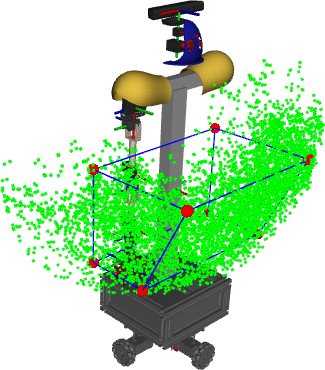
\includegraphics[width=4.50cm, height=5.5cm]{workSpace/ws_bb16.png}
	\caption{Vista lateral.}
	\end{subfigure}
	\caption{Espacio de trabajo acotado de un robot antropomórfico de 7DOF.}
\end{figure}

	En la siguiente tabla podemos observar los parametros que caracterizan el espacio de trabajo acotado para el brazo robótico de 7DOF.\\

\begin{table}[H]
\centering
\begin{tabular}{ |p{0.5cm}|p{1.5cm}|p{1.5cm}|}
 \hline
 \multicolumn{3}{|c|}{\textbf{PARAMÉTROS DEL ESPACIO DE TRABAJO}} \\
 \multicolumn{3}{|c|}{\textbf{DEL BRAZO ROBÓTICO}} \\
 \hline
 \multicolumn{3}{|c|}{\textbf{VERTICES}} \\
 \hline
    &  $P_1 $ & $[0.165837,   0.064973,  0.719878]$ \\
 \hline
    &  $P_2 $ & $[0.165837,  -0.57737,   0.719878]$ \\
 \hline
    &  $P_3 $ & $[0.426291,  -0.57737,   0.719878]$ \\
 \hline
    &  $P_4 $ & $[0.426291,   0.064973,  0.719878]$ \\
 \hline
    &  $P_5 $ & $[0.606291,   0.064973,  1.09449]$ \\
 \hline
    &  $P_6 $ & $[0.165837,   0.064973,  1.09449]$ \\
 \hline
    &  $P_7 $ & $[0.165837,  -0.57737,   1.09449]$ \\
 \hline
    &  $P_8 $ & $[0.165837,  -0.57737,   1.09449]$ \\
 \hline
 \multicolumn{3}{|c|}{\textbf{VOLUMEN}} \\
 \hline
 	&  $V[m^3]$ &   0.0838517      \\
 \hline
\end{tabular}
\caption{Tabla de características del espacio de trabajo para brazo robótico antropomórfico de 7DOF.}
\label{t_manip:9}
\end{table}	



%%%    ########################################   %%%%%%%%
%%% OBTENCIÓN DEL WS DEL BRAZO ROBOTICO DEL ALGORITMO
%%%    ########################################   %%%%%%%%


\newpage
	\section{Cinemática inversa Método Geométrico}
	El problema de la cinemática inversa consiste en dada una posición deseada $p(x, y, z, roll, pitch, yaw)$ encontrar el valor de cada una una de las juntas cinemáticas que lleven al brazo a la posición desea. Este problema suele ser uno de los más interesantes y complejos, dentro del estudio de la robótica. Es preciso mencionar que para llevar el efector final a cualquier posición y orientación deseada se requiere por lo menos un brazo robótico de 6DOF. En el desarrollo de este trabajo se plantea la resolución de la cinemática para un brazo robótico de 7DOF, lo cual suele aumentar el grado de complejidad en la resolución del problema.\\

\begin{equation}
\begin{split}
	H = 
	\begin{bmatrix}
	R  &  0  \\
	0  &  1  \\ 
	\end{bmatrix}
\end{split}
\end{equation}

	El problema de la cinemática inversa consiste en encontrar una o todas las soluciones:\\

\begin{equation}
	T^{0}_{n}(q_1, q_2...  q_n) = H
\end{equation}	
	
	Donde \textit{H} representa la matriz de posición y orientación deseada del efector final. Por tanto $q_1... q_n$ son los valores de las respectivas juntas mecánicas. Representado de otra manera:\\ 

\begin{equation}
	f(q_1, q_2...  q_n) = f(x, y, z, roll, pitch, yaw) 
\end{equation}	


	Para abordar la resolución de dicho problema se hizo uso del concepto de \textit{desacople cinemático}. Utilizando este concepto se puede simplificar el problema del cálculo completo de la cinemática inversa. Por medio del desacople cinemático se pueden considerar de manera independiente el cálculo de la orientación inversa y el cálculo de la posición inversa.\\

	\subsection{Desacople cinemático}
	Como se ha mencionado con anterioridad el problema de la cinemática inversa puede resolverse por separado en la resolución de la orientación inversa y la posición inversa, para manipuladores de 6 DOF o más. Es importate mencionar que para utilizar esta metodología de resolución el manipulador debe poseer la configuración de \textit{muñeca esférica}. Es necesario partir de esta premisa puesto que la configuración de muñeca esférica implica que los tres últimos ejes de acción de intersectan en un punto llamado $O_c$. Además estos tres últimos ejes de acción pueden determinar la orientación del efector final sin que dependan del valor de las juntas cinemáticas anteriores.\\

\begin{equation}
	R^0_7(q_1,.....  ,q_7) = R 
\end{equation}

\begin{equation}
	o^0_7(q_1,.....  ,q_7) = o 
\end{equation}

	La suposición de una \textit{muñeca esférica} implica que los ejes $z_4$, $z_5$ y $z_6$ se intersectan en $o_c$. Como se observa en la figura [4.20] el origen del sistema $O_5$ coincide con el centro de la muñeca esférica $O_c$. Es importante resaltar que el movimiento de los tres últimos ejes no afecta la posición del centro de la muñeca $O_c$. 

\begin{figure}[H]
	\centering
	\begin{subfigure}[t]{.55\textwidth}
	\centering
	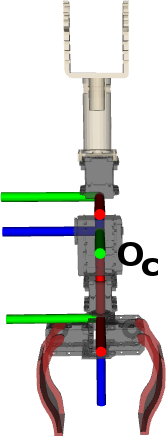
\includegraphics[width=2.50cm, height=7.0cm]{manipulator/wrist_center.png}
	\caption{Vista frontal.}
	\end{subfigure}%
	\begin{subfigure}[t]{.55\textwidth}
	\centering
	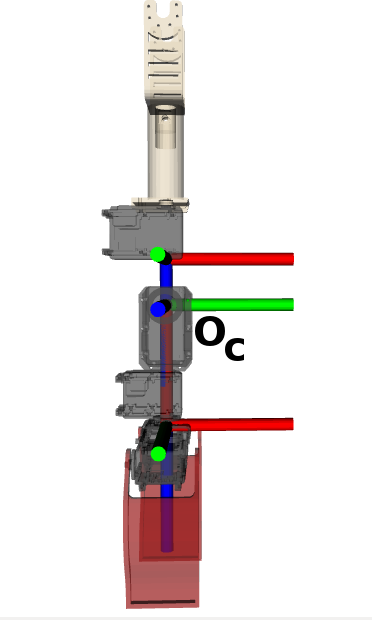
\includegraphics[width=5.00cm, height=7.0cm]{manipulator/wrist_center2.png}
	\caption{Vista lateral.}
	\end{subfigure}
	\caption{Centro de rotación de una muñeca esférica.}
\end{figure}

	El centro del efector final deseado podemos llamarlo \textit{o} y se puede obtener como la traslación $d_6$ a lo largo del eje \textit{x} a partir del punto $o^0_c$.\\

\begin{equation}
o = o^0_c + d_6 R \hat{x} 
\end{equation}

\begin{equation}
o^0_c = o - d_6 R \hat{x} 
\end{equation}

\begin{equation}
\begin{split}
	\begin{bmatrix}
	x_{oc}\\
	y_{oc}\\
	z_{oc} 
	\end{bmatrix}
	=
	\begin{bmatrix}
	x_{EE} - d_6 r_{13}\\
	y_{EE} - d_6 r_{23}\\
	z_{EE} - d_6 r_{33}
	\end{bmatrix}
\end{split} 
\end{equation}

	De la ecuación 4.13 podemos observar que para realizar el cálculo del punto que representa el centro de la muñena del manipulador solo debemos conocer el punto objetivo del efector final $P_{EE}$ y la orientación deseada \textit{R}. Utilizando la ecuación 4.13 calculamos el centro de la muñeca \textit{(punto en rojo)}. Posteriormente este punto servirá para calcular la cinemática inversa del manipulador quedando unicamente 4 valores de articulaciones por calcular.\\

\begin{figure}[H]
	\centering
	\begin{subfigure}[t]{.55\textwidth}
	\centering
	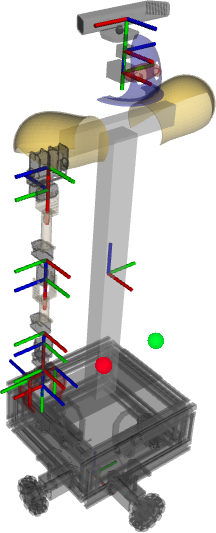
\includegraphics[width=3.50cm, height=7.0cm]{manipulator/wristCenter_yaw.png}
	\caption{Posición desea del efector final. (verde)}
	\end{subfigure}%
	\begin{subfigure}[t]{.55\textwidth}
	\centering
	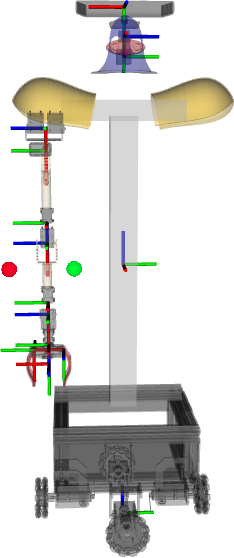
\includegraphics[width=3.00cm, height=7.0cm]{manipulator/wristCenter_yaw2.png}
	\caption{Posición del centro de la muñeca. (rojo)}
	\end{subfigure}
	\caption{Centro de la muñeca con rotación $\pi/2$.}
\end{figure}



\newpage
	\section{Cinemática inversa paquetería MoveIt}

	La paquetería de software \textit{moveIt} consiste en una serie de librerías enfocadas a las tareas de manipulación de objetos en la robótica. Los paquetes \textit{arm\_navigation} fueron diseñados con el objetivo especifico de ayudar en tareas de planeación de movimientos, generación de trayectorias y monitoreo del ambiente particularmente para los manipuladores del robot PR2.\cite{chitta2012moveit} La idea original al desarrollar la librería moveIt era generar planes de manipulación y trayectorias basándose información de un modelo del entorno. Dichos modelos del entorno se crean, comúnmente, utilizando la fusión de datos del sensor láser y de sensores estéreo colocados en los robots.\\


	El ambiente era representado como una mezcla de dos formatos:\\

	\begin{enumerate}
		\item{ Una red vóxelizada que representaba la mayor parte de los obstáculos en el medio ambiente. }

		\item{ Primitivas geométricas y modelos de mallas para representar objetos que habían sido reconocidos y registrado en el medio ambiente ambiente mediante rutinas de detección de objetos. }
	\end{enumerate}

	De esta manera la información del modelo del entorno sirve de entrada principal a los planificadores que constituyen la paquetería \textit{moveIt}.\\


	\textit{MoveIt!} incorpora herramientas para planeación de movimientos, cinemática, percepción 3D, control y navegación. Además provee una plataforma de uso fácil para desarrollo de aplicaciones robóticas avanzadas, permitiendo la evaluación de nuevos diseños de robots y la construcción de productos robóticos para su uso industrial, comercial y de investigación, entre otros. \textit{MoveIt!} Es el software de código abierto más usado para manipulación de robots.


	En la actualidad \textit{moveIt} proveé una interfaz genérica para la planeación de movimiento de manipuladores que puede ser integrada muy fácilmente en ROS. Esta interfaz permite la integración de diferentes tipos de planeadores de movimientos, por ejemplo:\\

	\begin{enumerate}
		\item{Planeadores aleatorizados. Open Motion Planning Library (OMPL).}

		\item{Planeadores basados en búsquedas. (SBPL)}

		\item{Librerías de optimización de trayectorias. (CHOMP)}

		\item{Librerías de optimización estocastica para la planeación de movimientos. (STOMP)}
	\end{enumerate} 

	La paquetería \textit{moveIt} permite personalizar el solucionador de cinemáticas para realizar cálculos más rápidos de la cinemática inversa. Utilizando para ello métodos numéricos. Una característica importante de la paquetería \textit{moveIt} es que para solucionar la cinemática inversa extrae de la información necesaria desde un archivo URDF (archivo estándar para descripción de robots en el formato aceptado por ROS).\\ 

	De esta manera se utilizó el archivo URDF que contiene la información con la descripción de las transformaciones entre los elementos del robot Justina. Para ello se creó un archivo extra que contiene unicamente la información de translaciones entre los elementos que constituyen los brazos del robot Justina. Como se muestra en la figura \ref{fig:desciption_arms1}.\\

	\begin{figure}[H]
	\centering
	\begin{subfigure}[t]{.55\textwidth}
		\centering
		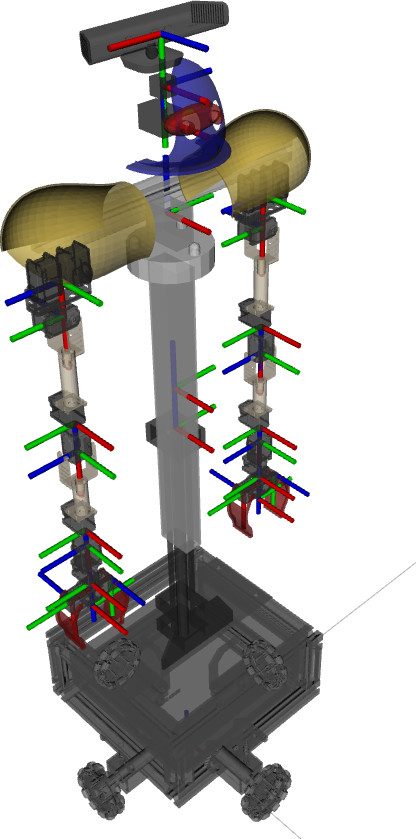
\includegraphics[width=3.50cm, height=7.0cm]{manipulator/DH_manipulators1.png}
		\caption{URDF descripción del robot Justina.}
	\end{subfigure}%
	\begin{subfigure}[t]{.55\textwidth}
		\centering
		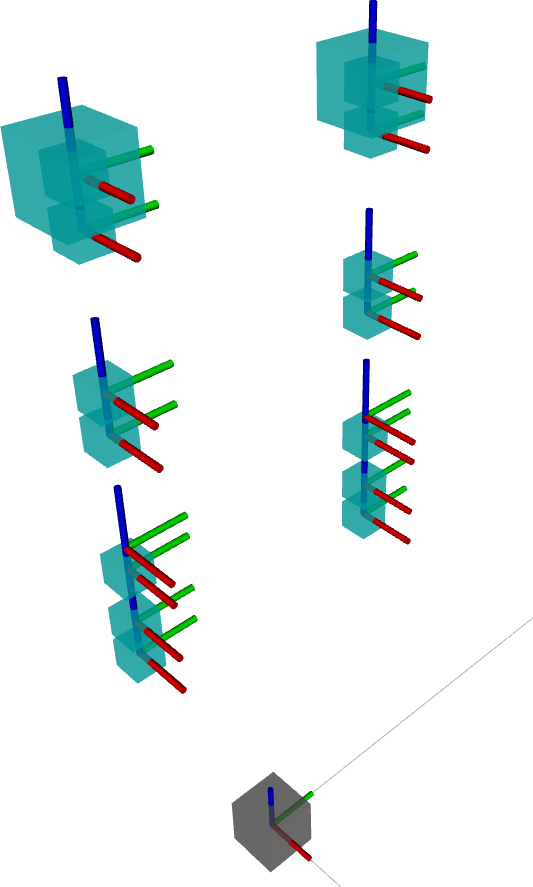
\includegraphics[width=3.50cm, height=6.0cm]{manipulator/moveIt_manipulators2.png}
		\caption{URDF descripción de las tranformaciones de los brazos del robot Justina.}
	\end{subfigure}
	\caption{Vista trimétrica del despliegue del robot Justina y sus respectivos manipuladores en el visualizador gráfico Rviz.}
	\label{fig:desciption_arms1}
	\end{figure}


	\begin{figure}[H]
	\begin{subfigure}[t]{.55\textwidth}
		\centering
		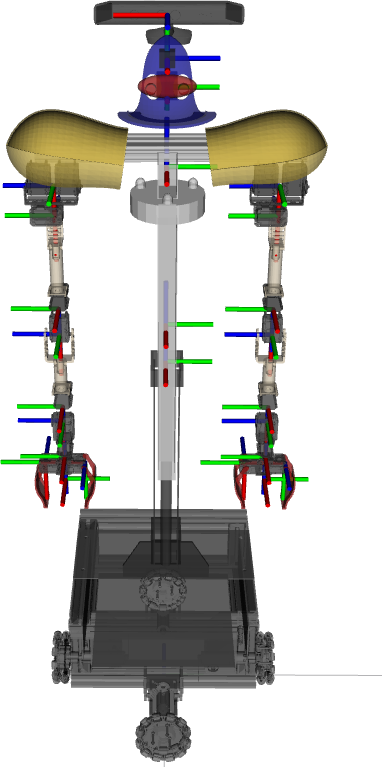
\includegraphics[width=3.50cm, height=7.0cm]{manipulator/DH_manipulators2.png}
		\caption{URDF descripción del robot Justina.}
	\end{subfigure}%
	\begin{subfigure}[t]{.55\textwidth}
		\centering
		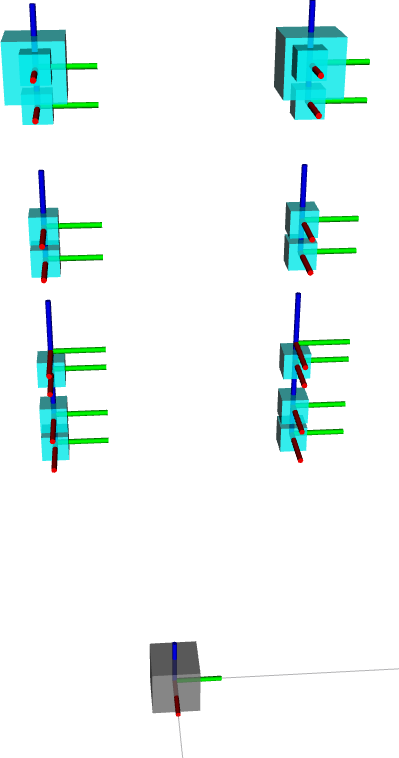
\includegraphics[width=3.50cm, height=6.0cm]{manipulator/moveIt_manipulators1.png}
		\caption{URDF descripción de las tranformaciones de los brazos del robot Justina.}
	\end{subfigure}
	\caption{Imagen de la comparación entre descripciones de los brazos del robot Justina.}
	\label{fig:desciption_arms2}
	\end{figure}

	Con la información del archivo URDF se creó un nuevo archivo que contiene la información de las relaciones entre los elementos que constituyen al robot Justina, tal documento es conocido como SURDF, por ser una descripción semántica del robot.\\

	Una vez que se generaron tales archivos se procedió a crear un modelo cinemático de los brazos del robot Justina. Tal modelo cinemático de los brazos nos da acceso a funciones para obtener la cinemática inversa, utilizando el solucionador de cinemática KLD integrado en la paquetería \textit{moveIt!}.\\

	Esta sección en particular tiene como objetivo comparar los ambos métodos de solución de la cinemática inversa del robot de servicio Justina. Por tanto en el presente trabajo se analiza y compara el tiempo de ejecución de ambos algoritmos. Y como característica extra se plantea una función de utilidad para evaluar la \textit{conveniencia} de utilizar un algoritmo u otro.\\

	\begin{figure}[H]
		\begin{minipage}{18cm}	
		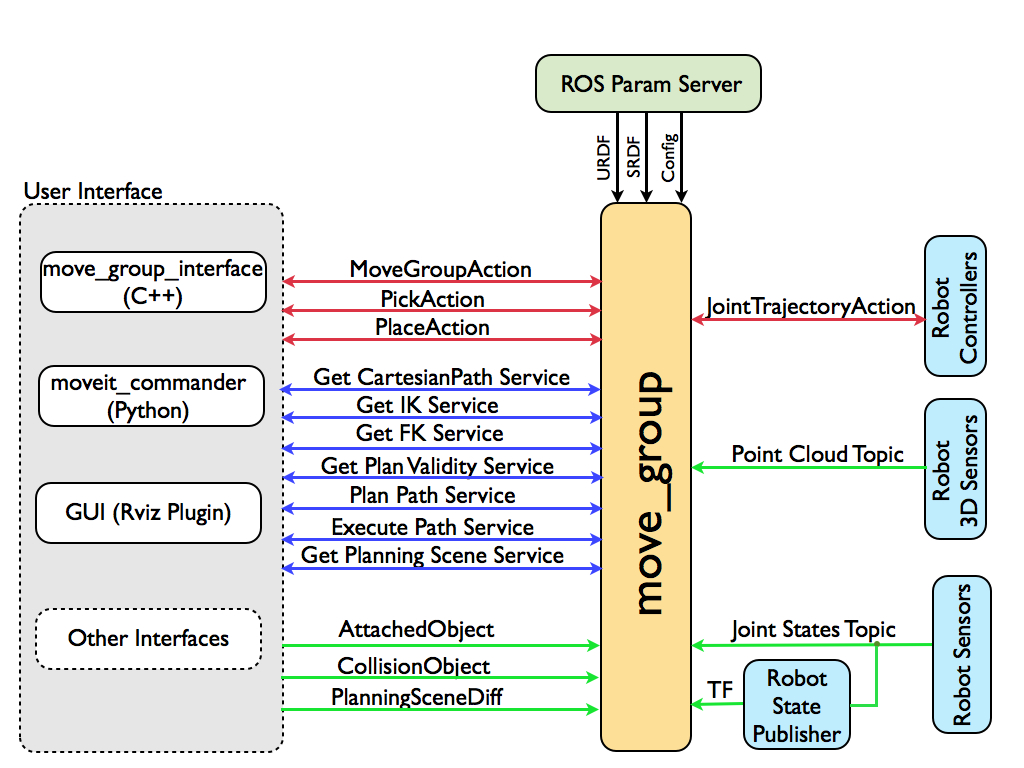
\includegraphics[scale=0.30]{ros/moveIt_structure.jpg}	
		\end{minipage}
		
		\begin{center}
		\caption{Imagen de la estructura de la paquetería \textit{moveIt!}.}
		\end{center}
	\end{figure}

	\section{Planteamiento de la función de costo para el cálculo de la cinemática inversa.}

	Sabemos que al resolver el problema de la cinemática inversa podemos obtener múltiples soluciones para una misma información de entrada $x, y, z, roll, pitch, yaw$. Por ello es importante determinar en que casos es conveniente tomar la información obtenida mediante un método geométrico o mediante un método iterativo. Por tal razón en el presente trabajo de tesis se plantea una función de costo que nos permita comparar y cuantificar ambos algoritmos de solución de cinemáticas.\\

	Para el planteamiento de la función de costo se tomaron en cuenta los siguientes aspectos:\\

	\begin{itemize}
		\item{Los valores de ángulos más alejados de cero implican un mayor gasto energético de los motores.}
		\item{Los ángulos de los motores 0 y 5, deben ser negativos para obtener un configuración de codo abajo y conservar una estructura antropomórfica de los brazos.}
	\end{itemize}

	\begin{equation}
	\begin{split}
		\epsilon = f(\theta_0, \theta_1, \theta_2, \theta_3, \theta_4, \theta_5, \theta_6) \cr
		\epsilon =  \sum_{i=0}^n |\theta_i| * \alpha
	\end{split}
	\end{equation}

	Donde $\alpha$ representa una ganancia que establecimos con un valor de 0.5. Para corregir el problema con la morfología de la toma de objetos se optó por restringir los valores de ángulos dentro del archivo que contiene la descripción del robot. De esta manera se realizaron los las pruebas llamando dos servicios para el cálculo de la cinemática inversa y evaluando la función de costo con la respuesta obtenida.\\


	\begin{figure}[H]
		\centering
		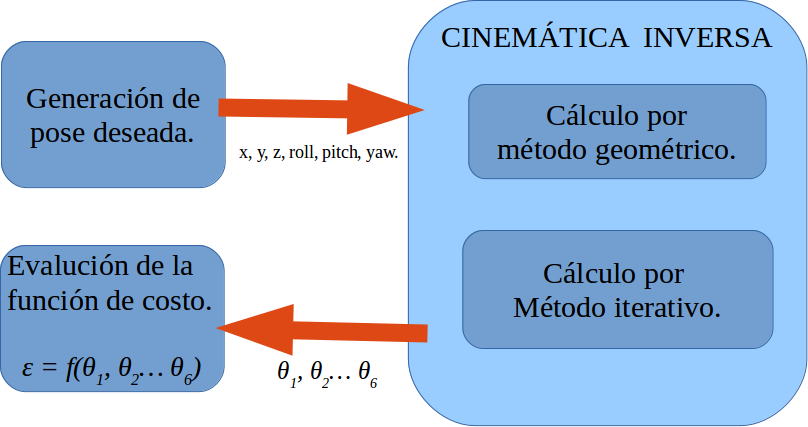
\includegraphics[width=11.00cm, height=5.5cm]{ros/cinematicaServices1.png}
		\caption{Imagen representativa de la comunicación entre módulos para evaluar la función de costo propuesta para el cálculo de la cinemática inversa.}
		\label{fig:cinematica_services}
	\end{figure}



